\documentclass{article}

\usepackage{fullpage}
\usepackage{url}
\usepackage{bbm}
\usepackage{graphicx}
\usepackage{amsmath}
\usepackage{physics}
\usepackage{mathtools}
\usepackage{bbold}
\usepackage{slashed}
\usepackage{pxfonts}
\usepackage{multicol}
\usepackage{mathptmx}
\usepackage{simplewick}
\usepackage{placeins}
\usepackage{booktabs}
\usepackage{tikz}
\usepackage[compat=1.1.0]{tikz-feynman}

\usepackage{lmodern}
\usepackage[T1]{fontenc}
\usepackage[fontsize=13.5pt]{fontsize}

\DeclareMathOperator{\erfi}{erfi}
\newcommand{\R}{\ensuremath{\mathbb{R}}}
\newcommand{\C}{\ensuremath{\mathbb{C}}}

\tikzset{
  counterterm/.style={
    circle,
    draw,
    inner sep=1pt,
    minimum size=3mm,
    path picture={
      \draw[black] 
      (path picture bounding box.south west) -- (path picture bounding box.north east)
      (path picture bounding box.south east) -- (path picture bounding box.north west);
    }
  }
}

\title{QFT1 Formulas}

\begin{document}
\maketitle

\section{Basics of QFT}
\subsection{Path integrals}
Definition:
\begin{equation}
    Z = \int \mathcal{D}\phi \, \exp\left( i \int d^4x \, \mathcal{L}[\phi, \partial_\mu\phi] \right) = \int \mathcal{D}\phi \, e^{iS[\phi]}
\end{equation}
Where
\begin{equation}
    \int \mathcal{D} x = \lim_{N\rightarrow\infty} \int \prod_{i=0}^N dx_i
\end{equation}
To get to that form from a correlation function:
\begin{itemize}
    \item Start from some correlation function between value at two times $t_0$ and $t_f$.
    \item Discretize time into $N$ intervals of $\Delta t = (t_f - t_0)/N$, such that $t_N = t_f$.
    \item Insert a complete set of states $\int d\phi_i |\phi_i\rangle \langle\phi_i| = \boldsymbol{1}$ at each time step $t_i$.
    \item Evaluate the infinitesimal transition amplitudes $\langle \phi_{i+1} | e^{-iH\Delta t} | \phi_i \rangle$.
    \item Take the continuum limit $N \to \infty, \Delta t \to 0$, transforming the product of integrals into the functional measure $\mathcal{D}\phi$.
\end{itemize}
\subsection{Correlation functions}
\begin{equation}
    \langle \Omega | T\{\phi(x_1) \dots \phi(x_n)\} | \Omega \rangle = \frac{\int \mathcal{D}\phi \, \phi(x_1) \dots \phi(x_n) e^{iS[\phi]}}{\int \mathcal{D}\phi \, e^{iS[\phi]}}
\end{equation}
\subsubsection*{Time ordering operator}
Places operators with later times to the left of operators with earlier times.
\newline
For bosons:
\begin{equation}
    T\{\phi(x) \phi(y)\} = \begin{cases}
        \phi(x)\phi(y)\theta(x^0 - y^0) + \phi(y)\phi(x)\theta(y^0 - x^0) & \text{for bosons} \\
        \phi(x)\phi(y)\theta(x^0 - y^0) - \phi(y)\phi(x)\theta(y^0 - x^0) & \text{for fermions}
    \end{cases}
\end{equation}
\subsubsection*{Normal ordering operator}
Places all creation operators ($a^\dagger$) to the left of all annihilation operators ($a$). Its vacuum expectation value is exactly zero.
\subsubsection*{Vacuum state definitions}
\begin{itemize}
    \item $|0\rangle$: The vacuum state of the \textit{free} theory ($H_0 |0\rangle = 0$).
    \item $|\Omega\rangle$: The true, interacting vacuum state of the full Hamiltonian $H$.
\end{itemize}
\subsubsection*{Wick's theorem}
\begin{equation}
    T\{\phi_1 \dots \phi_n\} = N\{\phi_1 \dots \phi_n\} + \text{all possible contractions}
\end{equation}
Inside $\langle 0 | \dots | 0 \rangle$, only the fully contracted terms survive.

\subsection{Source}
A classical external field $J(x)$ added to the Lagrangian to probe the system: $\mathcal{L} \to \mathcal{L} + J(x)\phi(x)$.
\begin{equation}
    Z[J] = \int \mathcal{D}\phi e^{i \int d^4x \, (\mathcal{L} + J\phi)}
\end{equation}
Correlation functions are generated by taking functional derivatives of $Z[J]$ with respect to $J$:
\begin{equation}
    \langle \Omega | T\{\phi(x_1) \dots \phi(x_n)\} | \Omega \rangle = \left. \frac{(-i)^n}{Z[0]} \frac{\delta^n Z[J]}{\delta J(x_1) \dots \delta J(x_n)} \right|_{J=0}
\end{equation}

\subsection{Scattering}
The transition matrix can be split into unity + a scattering matrix
\begin{equation}
    S = \boldsymbol{1} + iT
\end{equation}
Scattering matrix (with scattering amplitude):
\begin{equation}
    \langle f | iT | i \rangle = (2\pi)^4 \delta^{(4)}(p_f - p_i) i\mathcal{M}
\end{equation}
Cross section:
\begin{equation}
    d\sigma = \frac{1}{2E_A 2E_B |v_A - v_B|} |\mathcal{M}|^2 d\Pi_{\text{LIPS}}
\end{equation}
where
\begin{equation}
    d\Pi_{\text{LIPS}} = (2\pi)^4 \delta^{(4)}(p_A + p_B - \sum p_f) \prod_f \frac{d^3p_f}{(2\pi)^3 2E_f}
\end{equation}
Effective potential (in the non relativistic limit with distinguishable particles):
\begin{equation}
    \bra{p'}iT\ket{p} = -i \tilde{V}(\vec{p}' - \vec{p})(2\pi)\delta(E_{p'} - E_p)
\end{equation}
\subsubsection*{Decay rate}
For a single particle of mass $M$ decaying into a final state $f$:
\begin{equation}
    d\Gamma = \frac{1}{2M} |\mathcal{M}|^2 d\Pi_{\text{LIPS}}
\end{equation}

\subsection{Lippmann-Schwinger equation}
Describes scattering states in quantum mechanics.
\begin{equation}
    \ket{\phi_{\pm}} = \ket{\phi_0} + \frac{1}{E_0 - H_0 \pm i\epsilon}V\ket{\phi_{\pm}}
\end{equation}
Where $\ket{\phi_0}$ is the eigenstate of the free Hamiltonian $H_0$ with eigenvalue $E_0$, $V$ is the interaction potential ($H = H_0 + V$), and the $\pm i\epsilon$ defines the boundary conditions (incoming/outgoing spherical waves).

\subsection{Schwinger-Dyson equations}
Steps:
\begin{itemize}
    \item Utilize the invariance of the path integral measure under an infinitesimal field shift $\phi(x) \to \phi(x) + \epsilon(x)$.
    \item This implies the functional integral of a total derivative is zero: $\int \mathcal{D}\phi \frac{\delta}{\delta \phi(x)} \left( e^{iS[\phi]} \dots \right) = 0$.
    \item Expand the derivative to relate correlation functions of different orders.
\end{itemize}
Example - the $\phi^4$ equations:
\begin{itemize}
    \item Start with the identity: $\int \mathcal{D}\phi \frac{\delta}{\delta \phi(x)} \left( \phi(y) e^{iS[\phi]} \right) = 0$.
    \item Apply the functional derivative: $\int \mathcal{D}\phi \left( \delta^{(4)}(x-y) + i \phi(y) \frac{\delta S}{\delta \phi(x)} \right) e^{iS[\phi]} = 0$.
    \item Substitute the classical equation of motion $\frac{\delta S}{\delta \phi(x)} = -(\Box_x + m^2)\phi(x) - \frac{\lambda}{3!}\phi^3(x)$.
    \item Divide by $Z[0]$ to yield the time-ordered expectation value relation:
\end{itemize}
\begin{equation}
    (\Box_x + m^2)\langle \Omega | T\{\phi(x)\phi(y)\} | \Omega \rangle + \frac{\lambda}{3!}\langle \Omega | T\{\phi(x)^3\phi(y)\} | \Omega \rangle = -i\delta^{(4)}(x-y)
\end{equation}

\subsection{Ward-Takahashi identities}
Steps:
\begin{itemize}
    \item Assume a continuous symmetry in the Lagrangian (e.g., local gauge invariance).
    \item Perform a local change of variables in the path integral corresponding to the symmetry transformation.
    \item Demand that the path integral remains invariant, extracting the quantum analogue of Noether's current conservation.
\end{itemize}
Example - Complex $\phi^4$ / QED (Global $U(1)$):
\begin{itemize}
    \item Perform a local transformation $\phi(x) \to e^{i\alpha(x)}\phi(x) \approx \phi(x) + i\alpha(x)\phi(x)$.
    \item The variation of the action is $\delta S = -\int d^4x \, j^\mu(x) \partial_\mu \alpha(x)$.
    \item The path integral measure is invariant, so $\delta Z = 0$.
    \item Differentiate the invariant path integral $\int \mathcal{D}\phi \mathcal{D}\phi^* e^{iS} \phi(y_1)\dots\phi^*(z_1)$ with respect to $\alpha(x)$.
    \item Integration by parts yields the divergence of the current $\partial_\mu j^\mu$ inside the correlator, proportional to contact terms (delta functions) at the insertion points.
\end{itemize}
\begin{equation}
    \partial_\mu \langle T\{j^\mu(x) \phi(y_1) \dots \phi^*(z_1) \dots \} \rangle = -i \sum_k \delta^{(4)}(x - y_k) \langle \dots \rangle + i \sum_j \delta^{(4)}(x - z_j) \langle \dots \rangle
\end{equation}
\subsection{Composite operators}
\subsubsection*{Point Splitting Regularization}
When evaluating operators at the same spacetime point, e.g., $j^\mu = \bar{\psi}(x)\gamma^\mu\psi(x)$, products of fields at the exact same point are singular. We separate them by a small distance $\epsilon$:
\begin{equation}
    \bar{\psi}(x)\gamma^\mu\psi(x) \longrightarrow \lim_{\epsilon \to 0} \bar{\psi}(x+\epsilon/2) \gamma^\mu \exp\left( -ie \int_{x-\epsilon/2}^{x+\epsilon/2} A_\nu dz^\nu \right) \psi(x-\epsilon/2)
\end{equation}
The Wilson line exponential is required to maintain local gauge invariance.
\subsubsection*{Callan-Symanzik Equation}
For an $n$-point function with an insertion of a composite operator $\mathcal{O}(x)$, the equation picks up the anomalous dimension of the operator $\gamma_\mathcal{O}$:
\begin{equation}
    \left[ \mu \frac{\partial}{\partial \mu} + \beta(\lambda) \frac{\partial}{\partial \lambda} + n \gamma(\lambda) + \gamma_{\mathcal{O}}(\lambda) \right] G^{(n, \mathcal{O})}(x_1 \dots x_n; y) = 0
\end{equation}
\subsubsection*{Composite operators Renormalization}
Composite operators require their own renormalization. Because they share quantum numbers, different bare operators can mix under renormalization, requiring a mixing matrix $Z_{ij}$:
\begin{equation}
    \mathcal{O}_i^{(0)} = \sum_j Z_{ij} \mathcal{O}_j^{(R)}
\end{equation}
where $\mathcal{O}_i^{(0)}$ is the bare operator and $\mathcal{O}_j^{(R)}$ are the renormalized ones.

\newpage
\section{Regularization}
\subsection{Dimensional Regularization}
Steps:
\begin{itemize}
    \item Identify that the integral needs regularization
    \item change the dimension of the momentum integral $d_0 \rightarrow d$
    \item Use Feynman's trick to resolve the propegators into a single fraction
    \item Linearly change variables to complete the square in the denominator $l = p + \cdots$
    \item Name the remaining part of the denominator $\Delta$
    \item Remove odd powers of $l$
    \item Perform Wick's rotation $l^0 \rightarrow il_E^0$
    \item Split by powers of $l$ and use the known integrals:
    \begin{equation}
        \frac{d^dl_E}{(2\pi)^d} \frac{1}{(l_E^2 + \Delta)^n} = \frac{1}{(4\pi)^\frac{d}{2}}\frac{\Gamma\left(n - \frac{d}{2}\right)}{\Gamma(n)}\Delta^{\frac{d}{2} - n}
    \end{equation}
    \begin{equation}
        \frac{d^dl_E}{(2\pi)^d} \frac{l_E^2}{(l_E^2 + \Delta)^n} = \frac{d/2}{(4\pi)^\frac{d}{2}}\frac{\Gamma\left(n - \frac{d}{2} - 1\right)}{\Gamma(n)}\Delta^{\frac{d}{2} + 1 - n}
    \end{equation}
    \item Set the dimension $d = d_0 - \epsilon$ and use the approximation of $\Gamma$:
    \begin{equation}
        \Gamma(\epsilon) = \frac{1}{\epsilon} - \gamma + \mathcal{O}(\epsilon)
    \end{equation}
    and of powers of $\Delta$:
    \begin{equation}
        \Delta^{-\epsilon} = 1 - \epsilon \ln\Delta + \mathcal{O}(\epsilon^2)
    \end{equation}
\end{itemize}
Notes:
\begin{itemize}
    \item It preserves both Lorentz invariance and gauge invariance, making it the preferred method for gauge theories like QED and QCD.
    \item It struggles intrinsically with defining the $\gamma^5$ matrix since $\gamma^5$ is strictly a 4-dimensional object.
\end{itemize}
\subsection{Pauli-Villars Regularization}
Steps:
\begin{itemize}
    \item Introduce fictitious, heavy particles with mass $\Lambda$ to regulate high-momentum behavior by altering the propagator: $\frac{1}{k^2 - m^2} \to \frac{1}{k^2 - m^2} - \frac{1}{k^2 - \Lambda^2}$.
    \item Combine the fractions and remove vanishing terms. Only converging terms should remain.
    \item Use Feynman's trick and the subsequent steps from dimensional regularization above.
\end{itemize}
Notes:
\begin{itemize}
    \item Preserves local U(1) gauge invariance in QED but breaks non-Abelian gauge symmetries (QCD).
    \item The fictitious particles violate unitarity (negative probability/ghosts), so they must be removed by taking $\Lambda \to \infty$ after renormalization.
    \item Note: PV regularization fails for diagrams that diverge worse than logarithmically (e.g., the $\mathcal{O}(\lambda)$ 2-point function in $\phi^4$ which diverges linearly/quadratically because reducing the power of $k$ in the denominator by just 2 is insufficient), where dimensional regularization remains effective.
\end{itemize}
\newpage
\section{Renormalization}
\subsection{Superficial Degree of Divergence}
The total power of momentum in a loop integral.
Definition:
\begin{equation}
    D = d \cdot L - 2P = d + V\left(n \frac{d-2}{2} - d\right) - N \frac{d-2}{2}
\end{equation}
Where $d$ is the spacetime dimension, $L$ is the number of loops, $P$ is the number of internal propagators, $V$ is the number of vertices, and $N$ is the number of external legs. The coupling originates from a $\phi^n$ interaction. For a $\phi^4$ theory in $d=4$, this simplifies to $D = 4 - N$.
\subsubsection*{Diagram categorization}
\begin{itemize}
    \item $D > 0$: Superficially divergent (e.g., $D=2$ is quadratic divergence).
    \item $D = 0$: Superficially logarithmically divergent.
    \item $D < 0$: Superficially convergent (though it may contain divergent sub-diagrams).
\end{itemize}
\subsubsection*{Theory categorization}
\begin{itemize}
    \item \textbf{Super-renormalizable}: Only a finite number of Feynman diagrams are divergent (e.g., coupling has positive mass dimension).
    \item \textbf{Renormalizable}: Only a finite number of \textit{amplitudes} diverge; divergences appear at all loop orders but can be absorbed by a finite number of counterterms (e.g., coupling is dimensionless).
    \item \textbf{Non-renormalizable}: All amplitudes diverge at sufficiently high loop order; requires an infinite number of counterterms (e.g., coupling has negative mass dimension).
\end{itemize}
\subsection{Field Strength Renormalization}
The parameter $Z$ describing the probability that the bare field creates a 1-particle state from the vacuum. The renormalized field is defined as $\phi_R = \frac{1}{\sqrt{Z}}\phi_0$. It is determined by the derivative of the self-energy $\Sigma(p^2)$:
\begin{equation}
    Z = \left(1 - \left. \frac{\partial \Sigma(p^2)}{\partial p^2} \right|_{p^2=m^2}\right)^{-1}
\end{equation}
Using the K\"{a}ll\'{e}n-Lehmann spectral representation:
\begin{equation}
    \langle \Omega | T\{\phi(x)\phi(y)\} | \Omega \rangle = \int_0^\infty \frac{dM^2}{2\pi} \rho(M^2) \Delta_F(x-y; M^2)
\end{equation}
The spectral density $\rho(M^2)$ contains a delta function for the 1-particle state at the physical mass $m^2$. The field strength renormalization $Z = |\langle \Omega | \phi(0) | \lambda_0 \rangle|^2$ is the coefficient of this pole in momentum space:
\begin{equation}
    \Delta(p) = \frac{iZ}{p^2 - m^2 + i\epsilon} + \int_{\sim 4m^2}^\infty \frac{dM^2}{2\pi} \rho(M^2) \frac{i}{p^2 - M^2 + i\epsilon}
\end{equation}

\subsection{LSZ reduction formula}
Relates S-matrix elements to the time-ordered Green's functions of the interacting theory:
\begin{equation}
    \int \dots e^{i p \cdot x} \langle \Omega | T\{\phi(x_1) \dots \phi(x_n)\} | \Omega \rangle = \left( \prod_j \frac{i \sqrt{Z}}{p_j^2 - m^2} \right) \langle f | S | i \rangle
\end{equation}
\subsection{The optical theorem}
\begin{equation}
    2 \text{Im} \mathcal{M}(k_A, k_B \to k_A, k_B) = \sum_f \int d\Pi_f |\mathcal{M}(k_A, k_B \to f)|^2 = 2 E_{cm} p_{cm} \sigma_{\text{tot}}
\end{equation}
A direct consequence of the unitarity of the S-matrix ($S^\dagger S = \mathbb{1}$). It relates the imaginary part of the forward scattering amplitude to the total scattering cross-section.
\newline
The cross section on the right hand side involves a sum over all possible on-shell, physical multi-particle intermediate states that the initial particles can annihilate into. It serves as a mathematical statement of the conservation of probability in scattering processes.
\subsection{Renormalized perturbation theory}
(This is how we actually calcualte things):
\begin{itemize}
    \item Make sure the Lagrangian has all possible terms, allowed by symmetries.
    \item Express the bare Lagrangian in terms of renormalized fields, masses, and couplings ($\phi_0 = Z^{1/2}\phi$, $m_0 = Z_m m$, etc.).
    \item Define the physical masses and couplings, and split the Lagrangian to create counterterms.
    \item Treat the counterterms as new interaction vertices in Feynman diagrams.
    \item Choose a renormalization scheme (e.g., MS, $\overline{\text{MS}}$, or on-shell) to specify the renormalization conditions.
    \item Calculate the physical parameters based on their defitions, and use their definition to fix the counterterms.
    \item Write down the final expression using these counterterms.
\end{itemize}
\subsubsection*{Renormalization schemes}
\begin{itemize}
    \item \textbf{On-Shell Scheme:} Counterterms are chosen such that the renormalized mass $m$ is exactly the physical pole mass, and the field strength renormalization yields $Z=1$. This enforces $\Sigma(m^2) = 0$ and $\left.\frac{d\Sigma}{dp^2}\right|_{p^2=m^2} = 0$.
    \item \textbf{MS (Minimal Subtraction):} Counterterms are chosen to exactly cancel the $1/\epsilon$ poles arising in dimensional regularization, and nothing else.
    \item \textbf{$\overline{\text{MS}}$ (Modified Minimal Subtraction):} Counterterms cancel the $1/\epsilon$ pole along with the ubiquitous constants $\ln(4\pi)$ and the Euler-Mascheroni constant $\gamma_E$ that always naturally accompany the pole.
\end{itemize}
\subsection{The beta function}
The $\beta$ function encodes the running of the coupling constant $\lambda$ with the energy scale $\mu$.
\begin{equation}
    \beta(\lambda) = \mu \frac{\partial \lambda}{\partial \mu} = \frac{\partial \lambda}{\partial \ln \mu}
\end{equation}
\subsubsection*{The Callan–Symanzik Equation}
Describes how the $n$-point Green's functions shift under a change in the renormalization scale $\mu$:
\begin{equation}
    \left[ \mu \frac{\partial}{\partial \mu} + \beta(\lambda) \frac{\partial}{\partial \lambda} + n \gamma(\lambda) \right] G^{(n)}(x_1 \dots x_n; \mu, \lambda) = 0
\end{equation}
where $\gamma(\lambda) = \frac{1}{2} \mu \frac{\partial}{\partial \mu} \ln Z$ is the anomalous dimension of the field.
\subsubsection*{Classification of theories by beta function}
\begin{itemize}
    \item $\beta(\lambda) < 0$: The coupling decreases at high energies (Asymptotic Freedom). Characteristic of Non-Abelian gauge theories like QCD.
    \item $\beta(\lambda) > 0$: The coupling grows at high energies (Triviality / Landau pole). Characteristic of QED and $\phi^4$ theory.
    \item $\beta(\lambda) = 0$: The coupling is scale invariant (Conformal Field Theory).
\end{itemize}
\subsection{The Renormalization Group}
\subsubsection*{Wilsonian effective action}
Instead of dealing with counterterms, one integrates out high-momentum degrees of freedom (from a cutoff $\Lambda$ down to a lower scale $\Lambda'$). 
\begin{equation}
    Z = \int_{0 < k < \Lambda} \mathcal{D}\phi \, e^{iS[\phi]} = \int_{0 < k < \Lambda'} \mathcal{D}\phi \, e^{iS_{\text{eff}}[\phi]}
\end{equation}
This integration generates an infinite number of new interactions in the effective action $S_{\text{eff}}$.
\subsubsection*{Wilsonian beta function}
Tracking the coefficients (couplings) of these generated operators as the cutoff is lowered yields the Wilsonian RG flow equations. Couplings correspond to Relevant ($D > 0$), Marginal ($D = 0$), or Irrelevant ($D < 0$) operators depending on if they grow, stay constant, or decay at low energies.
\begin{equation}
    \beta_{Wil}^I(g) = \Lambda \frac{\partial g^I}{\partial \Lambda} = \gamma^I_J g^J + \beta^I_{JK}g^Jg^K
\end{equation}
\subsubsection*{Renormalization group equation}
Describes the flow of couplings in model space as a function of the threshold energy. In $\phi^n$ theory:
\begin{equation}
\begin{gathered}
    \frac{\partial g_n}{\partial \Lambda} = \frac{1}{2}\int \frac{d^4p}{(2\pi)^4} \Bigg[
        \sum
        g_{k+1}(p_1, \dots, p_k, p)\delta(p_1 + \cdots + p_k + p)\frac{\partial K^{-1}(p^2)}{\partial \Lambda} \times \\ \times g_{n-k+1}(p_{k+1}, \dots, p_n, -p) - \frac{\partial K^{-1}}{\partial \Lambda}g_{n+2}(p_1, \dots, p_n, -p)
    \Bigg]
\end{gathered}
\end{equation}
\subsubsection*{Renormalization group flow}
Linearizing the Wilsonian beta function around a fixed point $g^*$:
\begin{equation}
    \lambda^I = g^I - g^{*I} \qquad \beta(g^*) = 0
\end{equation}
\begin{equation}
    \Lambda \frac{\partial}{\partial \Lambda}\lambda^J = \gamma^I_J\lambda^J
\end{equation}
Diagonalizing to solve the system of PDEs gives another set of couplings $g'^I$:
\begin{equation}
    \Lambda \frac{\partial}{\partial \Lambda}\lambda'^I = \gamma^I\lambda'^I
\end{equation}
\begin{itemize}
    \item $\gamma^I > 0 \rightarrow$ Irrelevant
    \item $\gamma^I < 0 \rightarrow$ Relevant
\end{itemize}

\newpage
\section{Known Theories}
Theories that we saw in class
\subsection{Bare propagators by field}
Scalar:
\begin{equation}
    \Delta_F(p) = \frac{i}{p^2 - m_0^2 + i\epsilon} \\
\end{equation}
Dirac Fermion:
\begin{equation}
    S_F(p) = \frac{i(\slashed{p} + m_0)}{p^2 - m_0^2 + i\epsilon} \\
\end{equation}
Photon:
\begin{equation}
    D_F^{\mu\nu}(p) = \frac{-i}{p^2 + i\epsilon}\left(
        \eta^{\mu\nu} - (1 - \xi)\frac{p^\mu p^\nu}{p^2}
    \right)
\end{equation}
Photon (Feynman gauge, $\xi=1$):
\begin{equation}
    D_F^{\mu\nu}(p) = \frac{-i\eta^{\mu\nu}}{p^2 + i\epsilon}
\end{equation}
\subsection{$2 \rightarrow 2$ scattering and Mandelstam variables}
Mandelstam variables:
\begin{align}
    s &= (p_1 + p_2)^2 = (p_3 + p_4)^2 \\
    t &= (p_1 - p_3)^2 = (p_2 - p_4)^2 \\
    u &= (p_1 - p_4)^2 = (p_2 - p_3)^2
\end{align}
Note: $s + t + u = \sum_{i=1}^4 m_i^2$.
\subsection{Real scalar $\phi^4$ theory}
\subsubsection*{Full Bare Lagrangian}
\begin{equation}
    \mathcal{L} = \frac{1}{2}(\partial_\mu \phi)(\partial^\mu \phi) - \frac{1}{2}m^2\phi^2 - \frac{\lambda}{4!}\phi^4
\end{equation}
\subsubsection*{Symmetries}
Poincar\'{e} invariance, discrete $\mathbb{Z}_2$ parity ($\phi \to -\phi$).
\subsubsection*{Equations of Motion}
\begin{equation}
    (\Box + m^2)\phi + \frac{\lambda}{3!}\phi^3 = 0
\end{equation}
\subsubsection*{Superficial Degree of Divergence}
\begin{equation}
    D = 4 - N
\end{equation}
Where $N$ is the number of external legs.
\subsubsection*{Feynman rules}
\begin{center}
\begin{tabular}{|c|c|c|}
\hline
\textbf{Element} & \textbf{Position Space} & \textbf{Momentum Space} \\ \hline
Propagator & $\Delta_F(x-y)$ & $\frac{i}{p^2 - m^2 + i\epsilon}$ \\ \hline
Vertex & $-i\lambda \int d^4x$ & $-i\lambda (2\pi)^4\delta^{(4)}(\sum p)$ \\ \hline
External line & $1$ & $1$ \\ \hline
\end{tabular}
\end{center}
\subsubsection*{Counter terms and Renormalized Lagrangian}
\begin{equation}
    \mathcal{L} = \frac{1}{2}(\partial_\mu \phi_R)^2 - \frac{1}{2}m^2\phi_R^2 - \frac{\lambda}{4!}\phi_R^4 + \frac{1}{2}\delta_Z (\partial_\mu \phi_R)^2 - \frac{1}{2}\delta_m \phi_R^2 - \frac{\delta_\lambda}{4!}\phi_R^4
\end{equation}
Counterterm Propagator insertion: $i(p^2 \delta_Z - \delta_m)$ \\
Counterterm Vertex: $-i\delta_\lambda$
\subsubsection*{On-Shell Renormalization}
We fix the physical mass $m$ and field strength $Z=1$ by demanding the propagator has a pole at $p^2=m^2$ with residue $1$:
\begin{equation}
    \Sigma_R(m^2) = 0, \qquad \left.\frac{d\Sigma_R}{dp^2}\right|_{p^2=m^2} = 0
\end{equation}
\subsubsection*{Full Propagator}
After on-shell renormalization, the renormalized self-energy $\Sigma_R(p^2)$ vanishes at the mass shell, along with its first derivative. The full, exact propagator is:
\begin{equation}
    D_R(p^2) = \frac{i}{p^2 - m^2 - \Sigma_R(p^2 + i\epsilon)}
\end{equation}
Near the mass shell ($p^2 \approx m^2$), the full propagator behaves exactly like the free propagator:
\begin{equation}
    D_R(p^2) \xrightarrow{p^2 \to m^2} \frac{i}{p^2 - m^2 + i\epsilon}
\end{equation}
\subsubsection*{Interactions \& Correlation Functions}
\begin{itemize}
    \item \textbf{1-point:} $\langle \phi \rangle = 0$.
    \item \textbf{3-point (and any odd n-point):} Identically zero ($\langle \Omega | T\phi(x)\phi(y)\phi(z) | \Omega \rangle = 0$) due to exact $\mathbb{Z}_2$ parity.
    \item \textbf{4-point ($2 \to 2$ scattering):} Given by the 1PI 4-point vertex function $\Gamma^{(4)}(s, t, u)$. To one loop:
    \begin{equation}
        -i\mathcal{M} = -i\lambda + (-i\lambda)^2 [ iV(s) + iV(t) + iV(u) ] - i\delta_\lambda
    \end{equation}
    Where (before renormalization):
    \begin{equation}
        V(p^2) = \frac{1}{32\pi^2} \int_0^1 dx \left(
            \frac{2}{\epsilon} - \gamma - \ln\frac{m^2 - x(1-x)p^2}{4\pi} + \mathcal{O}(\epsilon)
        \right)
    \end{equation}
    And using on-shell renormalization conditions
    \begin{equation}
        \lambda_p = -i\mathcal{M}(p^i_0) \qquad p^i_0 = (m, \vec{0})
    \end{equation}
    \begin{equation}
        s = 4m^2, t = u = 0
    \end{equation}
    Gives:
    \begin{equation}
    \begin{gathered}
        -\mathcal{M} = \lambda_p + \lambda_p^2\left[V(s) + V(t) + V(u) - V(4m^2) - 2V(0)\right] = \\ =
        \lambda_p + \frac{\lambda_p^2}{32\pi^2}\int_0^1 dx\left[
            \ln\frac{m^2 - (1-x)s}{m^2 - x(1-x)4m^2} +
            \ln\frac{m^2 - (1-x)t}{m^2} +
            \ln\frac{m^2 - (1-x)u}{m^2}
        \right]
    \end{gathered}
    \end{equation}
\end{itemize}
\subsubsection*{Diagrams}
Tree $2 \to 2$ diagram
\begin{center}
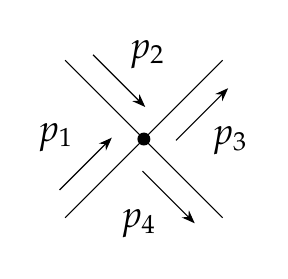
\begin{tikzpicture}[baseline=(current bounding box.center)]
  \begin{feynman}
    \vertex[dot] (v) at (0,0) {};
    \vertex (i1) at (-1, -1);
    \vertex (i2) at (-1, 1);
    \vertex (f1) at (1, 1);
    \vertex (f2) at (1, -1);
    \draw[plain, momentum=$p_1$] (i1) -- (v);
    \draw[plain, momentum=$p_2$] (i2) -- (v);
    \draw[plain, momentum'=$p_3$] (v) -- (f1);
    \draw[plain, momentum'=$p_4$] (v) -- (f2);
  \end{feynman}
\end{tikzpicture}
\end{center}
$2 \rightarrow 2$ scattering: S, T, and U channels:
\begin{center}
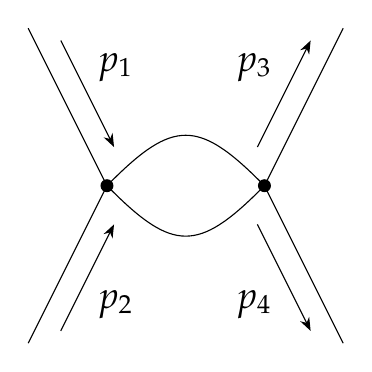
\begin{tikzpicture}[baseline=(current bounding box.center)]
  \begin{feynman}
    \vertex[dot] (v1) at (-1,0) {};
    \vertex[dot] (v2) at (1,0) {};
    \vertex (i1) at (-2, -2);
    \vertex (i2) at (-2, 2);
    \vertex (f1) at (2, 2);
    \vertex (f2) at (2, -2);
    \draw[plain, momentum=$p_1$] (i2) -- (v1);
    \draw[plain, momentum'=$p_2$] (i1) -- (v1);
    \draw[plain, momentum=$p_3$] (v2) -- (f1);
    \draw[plain, momentum'=$p_4$] (v2) -- (f2);
    \draw[plain] (v1) to[out=45, in=135, looseness=1.5] (v2);
    \draw[plain] (v1) to[out=-45, in=-135, looseness=1.5] (v2);
  \end{feynman}
\end{tikzpicture}
\hspace{1cm}
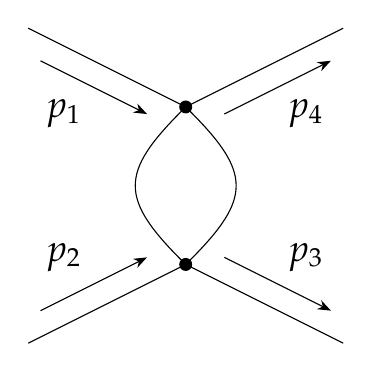
\begin{tikzpicture}[baseline=(current bounding box.center)]
  \begin{feynman}
    \vertex[dot] (v1) at (0,-1) {};
    \vertex[dot] (v2) at (0,1) {};
    \vertex (i1) at (-2, -2);
    \vertex (i2) at (-2, 2);
    \vertex (f1) at (2, -2);
    \vertex (f2) at (2, 2);
    \draw[plain, momentum'=$p_1$] (i2) -- (v2);
    \draw[plain, momentum=$p_2$] (i1) -- (v1);
    \draw[plain, momentum=$p_3$] (v1) -- (f1);
    \draw[plain, momentum'=$p_4$] (v2) -- (f2);
    \draw[plain] (v1) to[out=45, in=-45, looseness=1.5] (v2);
    \draw[plain] (v1) to[out=135, in=-135, looseness=1.5] (v2);
  \end{feynman}
\end{tikzpicture}
\hspace{1cm}
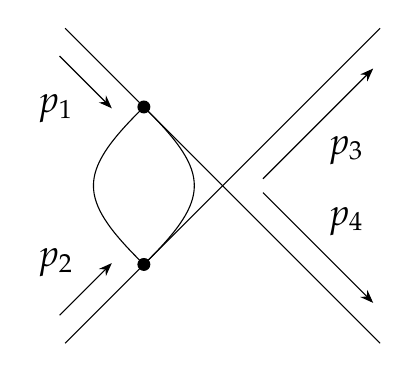
\begin{tikzpicture}[baseline=(current bounding box.center)]
  \begin{feynman}
    \vertex (i1) at (-2, -2);
    \vertex (i2) at (-2, 2);
    \vertex (f1) at (2, 2);
    \vertex (f2) at (2, -2);
    \vertex[dot] (v1) at (-1, 1) {};
    \vertex[dot] (v2) at (-1, -1) {};
    \vertex (v0) at (0,0);
    \draw[plain, momentum'=$p_1$] (i2) -- (v1);
    \draw[plain, momentum=$p_2$] (i1) -- (v2);
    \draw[plain, momentum'=$p_3$] (v0) -- (f1);
    \draw[plain, momentum=$p_4$] (v0) -- (f2);
    \draw[plain] (v2) -- (v0);
    \draw[plain] (v1) -- (v0);
    \draw[plain] (v2) to[out=45, in=-45, looseness=1.5] (v1);
    \draw[plain] (v2) to[out=135, in=-135, looseness=1.5] (v1);
  \end{feynman}
\end{tikzpicture}
\end{center}
1-loop correction diagrams (Tadpole Self-Energy and Vertex Correction):
\begin{center}
\begin{tikzpicture}[baseline=(current bounding box.center)]
  \begin{feynman}
    \vertex (a);
    \vertex [right=1.5cm of a] (b);
    \vertex [right=1.5cm of b] (c);
    \diagram* {
      (a) -- (b) -- (c),
      (b) -- [half left, looseness=1.5, momentum=$k$] (b)
    };
  \end{feynman}
\end{tikzpicture}
\hspace{2cm}
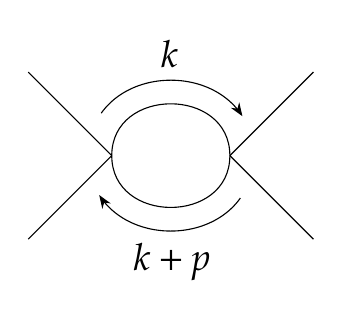
\begin{tikzpicture}[baseline=(current bounding box.center)]
  \begin{feynman}
    \vertex (a); \vertex [below right=of a] (b);
    \vertex [below left=of b] (c);
    \vertex [right=1.5cm of b] (d);
    \vertex [above right=of d] (e);
    \vertex [below right=of d] (f);
    \diagram* {
      (a) -- (b) -- (c),
      (b) -- [half left, momentum=$k$] (d) -- [half left, momentum=$k+p$] (b),
      (d) -- (e), (d) -- (f)
    };
  \end{feynman}
\end{tikzpicture}
\end{center}
Counter terms:
\begin{center}
\begin{tikzpicture}[baseline=(current bounding box.center)]
  \begin{feynman}
    \vertex (v1) at (-1,0) {};
    \vertex (v2) at (1,0) {};
    \vertex[counterterm] (v0) at (0,0) {};
    \draw[plain] (v1) -- (v0);
    \draw[plain] (v0) -- (v2);
  \end{feynman}
\end{tikzpicture}
\hspace{1cm}
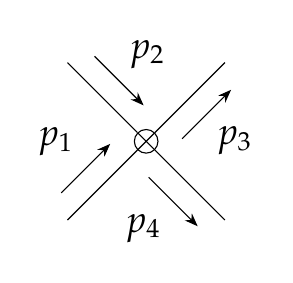
\begin{tikzpicture}[baseline=(current bounding box.center)]
  \begin{feynman}
    \vertex[counterterm] (v) at (0,0) {};
    \vertex (i1) at (-1, -1);
    \vertex (i2) at (-1, 1);
    \vertex (f1) at (1, 1);
    \vertex (f2) at (1, -1);
    \draw[plain, momentum=$p_1$] (i1) -- (v);
    \draw[plain, momentum=$p_2$] (i2) -- (v);
    \draw[plain, momentum'=$p_3$] (v) -- (f1);
    \draw[plain, momentum'=$p_4$] (v) -- (f2);
  \end{feynman}
\end{tikzpicture}
\end{center}
\subsubsection*{Beta Function}
\begin{equation}
    \beta(\lambda) = \frac{3\lambda^2}{16\pi^2}
\end{equation}
\subsection{Complex scalar $\phi^4$ theory}
\subsubsection*{Full Bare Lagrangian}
\begin{equation}
    \mathcal{L} = (\partial_\mu \phi^\dagger)(\partial^\mu \phi) - m^2\phi^\dagger \phi - \frac{\lambda}{4}(\phi^\dagger \phi)^2
\end{equation}
\subsubsection*{Symmetries}
Poincar\'{e} invariance, Global $U(1)$ charge ($\phi \to e^{i\alpha}\phi$), Charge Conjugation $C$ ($\phi \leftrightarrow \phi^\dagger$).
\subsubsection*{Equations of Motion}
\begin{equation}
    (\Box + m^2)\phi + \frac{\lambda}{2}(\phi^\dagger \phi)\phi = 0
\end{equation}
\subsubsection*{Superficial Degree of Divergence}
\begin{equation}
    D = 4 - N
\end{equation}
Where $N$ is the number of external legs.
\subsubsection*{Feynman rules}
\begin{center}
\begin{tabular}{|c|c|c|}
\hline
\textbf{Element} & \textbf{Position Space} & \textbf{Momentum Space} \\ \hline
Directed Propagator & $\Delta_F(x-y)$ & $\frac{i}{p^2 - m^2 + i\epsilon}$ (follows arrow) \\ \hline
Vertex (2 in, 2 out) & $-i\lambda \int d^4x$ & $-i\lambda (2\pi)^4\delta^{(4)}(\sum p)$ \\ \hline
\end{tabular}
\end{center}
\subsubsection*{Counter terms and Renormalized Lagrangian}
\begin{equation}
    \mathcal{L}_{CT} = \delta_Z (\partial_\mu \phi^\dagger)(\partial^\mu \phi) - \delta_m \phi^\dagger \phi - \frac{\delta_\lambda}{4}(\phi^\dagger \phi)^2
\end{equation}
Self-energy counterterm: $i(p^2\delta_Z - \delta_m)$ \\
4-point counterterm: $-i\delta_\lambda$
\subsubsection*{On-Shell Renormalization}
Similar to real $\phi^4$, we demand the pole resides at the physical mass $m^2$ with residue $1$:
\begin{equation}
    \Sigma_R(m^2) = 0, \qquad \left.\frac{d\Sigma_R}{dp^2}\right|_{p^2=m^2} = 0
\end{equation}
And we fix the coupling at threshold: $\lambda_p = -i\mathcal{M}(s=4m^2, t=0, u=0)$.
\subsubsection*{Full Propagator}
After on-shell renormalization, the full exact propagator is:
\begin{equation}
    D_R(p^2) = \frac{i}{p^2 - m^2 - \Sigma_R(p^2 + i\epsilon)} \xrightarrow{p^2 \to m^2} \frac{i}{p^2 - m^2 + i\epsilon}
\end{equation}
Only the mixed correlator $\langle \Omega | T\phi^\dagger(x) \phi(y) | \Omega \rangle$ is non-zero. $\langle \phi(x)\phi(y) \rangle = 0$ due to charge conservation.
\subsubsection*{Ward-Takahashi Identity / Noether Current}
Global $U(1)$ yields the conserved current $j^\mu = i(\phi^\dagger \partial^\mu \phi - \phi \partial^\mu \phi^\dagger)$ with $\partial_\mu j^\mu = 0$. In correlation functions, this implies the Ward identity:
\begin{equation}
    \partial_\mu \langle T\{j^\mu(x) \phi(y_1) \dots \phi^*(z_1) \dots \} \rangle = -i \sum_k \delta^{(4)}(x - y_k) \langle \dots \rangle + i \sum_j \delta^{(4)}(x - z_j) \langle \dots \rangle
\end{equation}
\subsubsection*{Interactions \& Correlation Functions}
\begin{itemize}
    \item \textbf{1-point:} $\langle \phi \rangle = 0$, by global $U(1)$ charge conservation.
    \item \textbf{3-point:} All 3-point correlation functions (e.g., $\langle \Omega | T\phi^\dagger(x) \phi(y) \phi(z) | \Omega \rangle$) are identically zero because they violate global $U(1)$ charge conservation. The sum of incoming and outgoing charges must be zero.
    \item \textbf{$2 \to 2$ scattering ($\phi \phi \to \phi \phi$):} Proceeds only via $t$ and $u$ channels (arrows must align continuously).
    \item \textbf{$2 \to 2$ scattering ($\phi \phi^* \to \phi \phi^*$):} Proceeds via $s$ and $t$ channels.
\end{itemize}
\subsubsection*{Diagrams}
Tree $2 \to 2$ scattering ($\phi \phi \to \phi \phi$), T and U channels:
\begin{center}
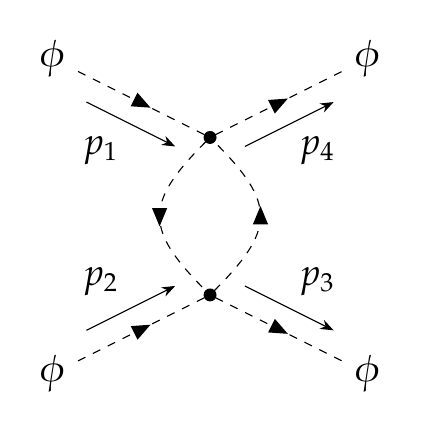
\begin{tikzpicture}[baseline=(current bounding box.center)]
  \begin{feynman}
    \vertex[dot] (v1) at (0,-1) {};
    \vertex[dot] (v2) at (0,1) {};
    \vertex (i1) at (-2, -2) {$\phi$};
    \vertex (i2) at (-2, 2) {$\phi$};
    \vertex (f1) at (2, -2) {$\phi$};
    \vertex (f2) at (2, 2) {$\phi$};
    \draw[charged scalar, momentum'=$p_1$] (i2) -- (v2);
    \draw[charged scalar, momentum=$p_2$] (i1) -- (v1);
    \draw[charged scalar, momentum=$p_3$] (v1) -- (f1);
    \draw[charged scalar, momentum'=$p_4$] (v2) -- (f2);
    \draw[charged scalar] (v1) to[out=45, in=-45, looseness=1.5] (v2);
    \draw[charged scalar] (v2) to[out=-135, in=135, looseness=1.5] (v1);
  \end{feynman}
\end{tikzpicture}
\hspace{1cm}
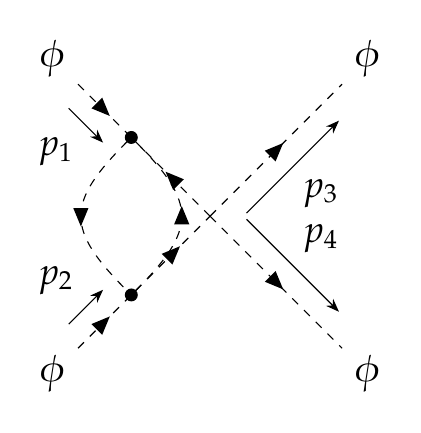
\begin{tikzpicture}[baseline=(current bounding box.center)]
  \begin{feynman}
    \vertex (i1) at (-2, -2) {$\phi$};
    \vertex (i2) at (-2, 2) {$\phi$};
    \vertex (f1) at (2, 2) {$\phi$};
    \vertex (f2) at (2, -2) {$\phi$};
    \vertex[dot] (v1) at (-1, 1) {};
    \vertex[dot] (v2) at (-1, -1) {};
    \vertex (v0) at (0,0);
    \draw[charged scalar, momentum'=$p_1$] (i2) -- (v1);
    \draw[charged scalar, momentum=$p_2$] (i1) -- (v2);
    \draw[charged scalar, momentum'=$p_3$] (v0) -- (f1);
    \draw[charged scalar, momentum=$p_4$] (v0) -- (f2);
    \draw[charged scalar] (v2) -- (v0);
    \draw[charged scalar] (v0) -- (v1);
    \draw[charged scalar] (v1) to[out=-135, in=135, looseness=1.5] (v2);
    \draw[charged scalar] (v2) to[out=45, in=-45, looseness=1.5] (v1);
  \end{feynman}
\end{tikzpicture}
\end{center}
Tree $2 \to 2$ scattering ($\phi \phi^* \to \phi \phi^*$), S and T channels:
\begin{center}
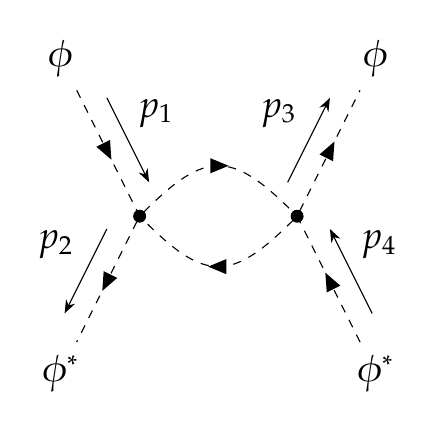
\begin{tikzpicture}[baseline=(current bounding box.center)]
  \begin{feynman}
    \vertex[dot] (v1) at (-1,0) {};
    \vertex[dot] (v2) at (1,0) {};
    \vertex (i1) at (-2, -2) {$\phi^*$};
    \vertex (i2) at (-2, 2) {$\phi$};
    \vertex (f1) at (2, 2) {$\phi$};
    \vertex (f2) at (2, -2) {$\phi^*$};
    \draw[charged scalar, momentum=$p_1$] (i2) -- (v1);
    \draw[charged scalar, momentum'=$p_2$] (v1) -- (i1);
    \draw[charged scalar, momentum=$p_3$] (v2) -- (f1);
    \draw[charged scalar, momentum'=$p_4$] (f2) -- (v2);
    \draw[charged scalar] (v1) to[out=45, in=135, looseness=1.5] (v2);
    \draw[charged scalar] (v2) to[out=-135, in=-45, looseness=1.5] (v1);
  \end{feynman}
\end{tikzpicture}
\hspace{1cm}
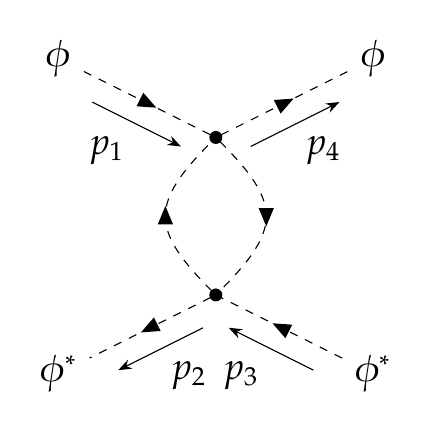
\begin{tikzpicture}[baseline=(current bounding box.center)]
  \begin{feynman}
    \vertex[dot] (v1) at (0,-1) {};
    \vertex[dot] (v2) at (0,1) {};
    \vertex (i1) at (-2, -2) {$\phi^*$};
    \vertex (i2) at (-2, 2) {$\phi$};
    \vertex (f1) at (2, -2) {$\phi^*$};
    \vertex (f2) at (2, 2) {$\phi$};
    \draw[charged scalar, momentum'=$p_1$] (i2) -- (v2);
    \draw[charged scalar, momentum=$p_2$] (v1) -- (i1);
    \draw[charged scalar, momentum=$p_3$] (f1) -- (v1);
    \draw[charged scalar, momentum'=$p_4$] (v2) -- (f2);
    \draw[charged scalar] (v2) to[out=-45, in=45, looseness=1.5] (v1);
    \draw[charged scalar] (v1) to[out=135, in=-135, looseness=1.5] (v2);
  \end{feynman}
\end{tikzpicture}
\end{center}
1-loop diagrams (Self Energy and Vertex Correction):
\begin{center}
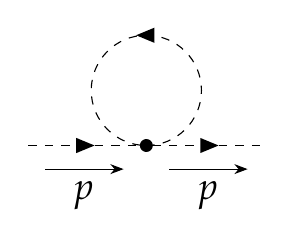
\begin{tikzpicture}[baseline=(current bounding box.center)]
  \begin{feynman}
    \vertex (v1) at (-1.5,0);
    \vertex[dot] (v2) at (0,0) {};
    \vertex (v3) at (1.5,0);
    \draw[charged scalar, momentum'=$p$] (v1) -- (v2);
    \draw[charged scalar, momentum'=$p$] (v2) -- (v3);
    \draw[charged scalar] (v2) arc[start angle=-90, end angle=270, radius=0.7cm];
  \end{feynman}
\end{tikzpicture}
\hspace{1.5cm}
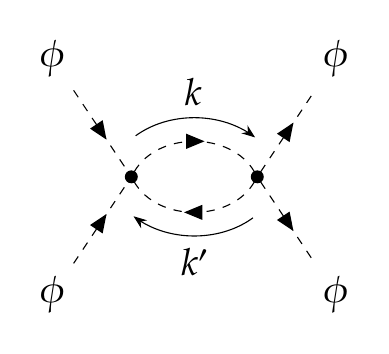
\begin{tikzpicture}[baseline=(current bounding box.center)]
  \begin{feynman}
    \vertex[dot] (v1) at (-0.8,0) {};
    \vertex[dot] (v2) at (0.8,0) {};
    \vertex (i1) at (-1.8, -1.5) {$\phi$};
    \vertex (i2) at (-1.8, 1.5) {$\phi$};
    \vertex (f1) at (1.8, 1.5) {$\phi$};
    \vertex (f2) at (1.8, -1.5) {$\phi$};
    \draw[charged scalar] (i2) -- (v1);
    \draw[charged scalar] (i1) -- (v1);
    \draw[charged scalar] (v2) -- (f1);
    \draw[charged scalar] (v2) -- (f2);
    \draw[charged scalar, momentum=$k$] (v1) to[out=60, in=120] (v2);
    \draw[charged scalar, momentum=$k'$] (v2) to[out=-120, in=-60] (v1);
  \end{feynman}
\end{tikzpicture}
\end{center}
Counter terms:
\begin{center}
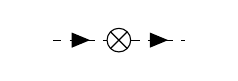
\begin{tikzpicture}[baseline=(current bounding box.center)]
  \begin{feynman}
    \vertex (v1) at (-1,0) {};
    \vertex (v2) at (1,0) {};
    \vertex[counterterm] (v0) at (0,0) {};
    \draw[charged scalar] (v1) -- (v0);
    \draw[charged scalar] (v0) -- (v2);
  \end{feynman}
\end{tikzpicture}
\hspace{1cm}
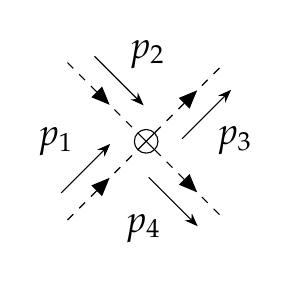
\begin{tikzpicture}[baseline=(current bounding box.center)]
  \begin{feynman}
    \vertex[counterterm] (v) at (0,0) {};
    \vertex (i1) at (-1, -1);
    \vertex (i2) at (-1, 1);
    \vertex (f1) at (1, 1);
    \vertex (f2) at (1, -1);
    \draw[charged scalar, momentum=$p_1$] (i1) -- (v);
    \draw[charged scalar, momentum=$p_2$] (i2) -- (v);
    \draw[charged scalar, momentum'=$p_3$] (v) -- (f1);
    \draw[charged scalar, momentum'=$p_4$] (v) -- (f2);
  \end{feynman}
\end{tikzpicture}
\end{center}
\subsubsection*{Beta Function}
\begin{equation}
    \beta(\lambda) = \frac{5\lambda^2}{16\pi^2}
\end{equation}
\subsection{Yukawa theory}
\subsubsection*{Full Bare Lagrangian}
(Note: $\phi^4$ term is \textit{required} for renormalizability because fermion box diagrams generate it).
\begin{equation}
    \mathcal{L} = \bar{\psi}(i\slashed{\partial} - m_f)\psi + \frac{1}{2}(\partial_\mu \phi)^2 - \frac{1}{2}m_s^2\phi^2 - g \bar{\psi}\psi\phi - \frac{\lambda}{4!}\phi^4
\end{equation}
\subsubsection*{Symmetries}
Poincar\'{e} invariance, Global $U(1)$ (Fermion number). Parity ($\psi \to \gamma^0 \psi, \phi \to -\phi$ if pseudoscalar).
\subsubsection*{Equations of Motion}
\begin{equation}
    (i\slashed{\partial} - m_f)\psi = g\phi\psi, \qquad (\Box + m_s^2)\phi = -g\bar{\psi}\psi - \frac{\lambda}{3!}\phi^3
\end{equation}
\subsubsection*{Superficial Degree of Divergence}
\begin{equation}
    D = 4 - \frac{3}{2}N_f - N_b
\end{equation}
Where $N_f$ is the number of external fermions, and $N_b$ is the number of external scalars.
\subsubsection*{Feynman rules}
\begin{itemize}
    \item Fermion Propagator: $\frac{i(\slashed{p}+m_f)}{p^2-m_f^2+i\epsilon}$
    \item Scalar Propagator: $\frac{i}{p^2-m_s^2+i\epsilon}$
    \item Yukawa Vertex: $-ig(2\pi)^4\delta^{(4)}(\sum p)$
\end{itemize}
\subsubsection*{Counter terms and Renormalized Lagrangian}
\begin{equation}
    \mathcal{L}_{CT} = \delta_{Z_f} \bar{\psi}i\slashed{\partial}\psi - \delta_{m_f} \bar{\psi}\psi + \frac{1}{2}\delta_{Z_s} (\partial\phi)^2 - \frac{1}{2}\delta_{m_s}\phi^2 - \delta_g \bar{\psi}\psi\phi - \frac{\delta_\lambda}{4!}\phi^4 + Y\phi
\end{equation}
Standard insertions for fermion line ($i(\slashed{p}\delta_{Z_f} - \delta_{m_f})$), scalar line ($i(p^2\delta_{Z_s} - \delta_{m_s})$), vertex ($-i\delta_g$), and the linear tadpole counterterm $Y\phi$.
\subsubsection*{On-Shell Renormalization}
We demand that the exact propagators have poles at their physical masses, with residue 1, and the vertex at zero momentum transfer yields the physical coupling $g$:
\begin{equation}
    \Sigma_{fR}(\slashed{p}=m_f) = 0, \qquad \left.\frac{d\Sigma_{fR}}{d\slashed{p}}\right|_{\slashed{p}=m_f} = 0
\end{equation}
\begin{equation}
    \Sigma_{sR}(p^2=m_s^2) = 0, \qquad \left.\frac{d\Sigma_{sR}}{dp^2}\right|_{p^2=m_s^2} = 0
\end{equation}
\begin{equation}
    -i\Gamma(p'-p=0) = -ig \qquad \text{(with on-shell fermions $p^2=p'^2=m_f^2$)}
\end{equation}
\subsubsection*{Full Propagators}
After on-shell renormalization, the full exact propagators are:
Fermion:
\begin{equation}
    S_{F,R}(p) = \frac{i}{\slashed{p} - m_f - \Sigma_{fR}(\slashed{p})} \xrightarrow{p^2 \to m_f^2} \frac{i}{\slashed{p} - m_f + i\epsilon}
\end{equation}
Scalar:
\begin{equation}
    D_{F,R}(p) = \frac{i}{p^2 - m_s^2 - \Sigma_{sR}(p^2)} \xrightarrow{p^2 \to m_s^2} \frac{i}{p^2 - m_s^2 + i\epsilon}
\end{equation}
\subsubsection*{Interactions \& Correlation Functions}
\begin{itemize}
    \item \textbf{1-point:} Fermion loops induce a scalar tadpole $\langle \phi \rangle \neq 0$. The linear counterterm $Y\phi$ is explicitly required to cancel it.
    \item \textbf{3-point:} The fundamental 3-point function is the $\psi\bar{\psi}\phi$ interaction, $\langle \Omega | T \psi(x) \bar{\psi}(y) \phi(z) | \Omega \rangle$, given by the 1PI vertex function $-i\Gamma(p',p)$. At tree level, this is simply $-ig$.
    \item \textbf{$2 \to 2$ Fermion scattering ($\psi \psi \to \psi \psi$):} Proceeds via $t$ and $u$ channel scalar exchange.
    \item \textbf{Effective Potential:} Generates an attractive Yukawa potential $V(r) = -\frac{g^2}{4\pi r}e^{-m_s r}$ in the non-relativistic limit.
\end{itemize}
\subsubsection*{Diagrams}
Vertex:
\begin{center}
\begin{tikzpicture}[baseline=(current bounding box.center)]
  \begin{feynman}
    \vertex[dot] (v1) at (0,0) {};
    \vertex (i1) at (-0.7, 1.4) {$\psi$};
    \vertex (i2) at (-0.7, -1.4) {$\psi$};
    \vertex (f2) at (1.5, 0) {$\phi$};
    \draw[fermion] (v1) -- (i1);
    \draw[fermion] (i2) -- (v1);
    \draw[scalar] (v1) -- (f2);
  \end{feynman}
\end{tikzpicture}
\end{center}
Tree $2 \to 2$ Fermion scattering ($\psi \psi \to \psi \psi$), T and U channels:
\begin{center}
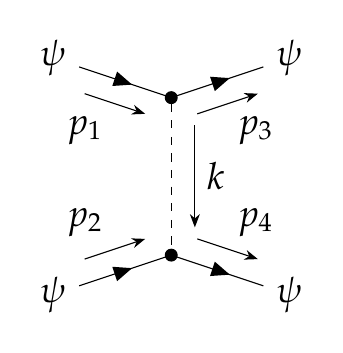
\begin{tikzpicture}[baseline=(current bounding box.center)]
  \begin{feynman}
    \vertex[dot] (v1) at (0,1) {};
    \vertex[dot] (v2) at (0,-1) {};
    \vertex (i1) at (-1.5, 1.5) {$\psi$};
    \vertex (f1) at (1.5, 1.5) {$\psi$};
    \vertex (i2) at (-1.5, -1.5) {$\psi$};
    \vertex (f2) at (1.5, -1.5) {$\psi$};
    \draw[fermion, momentum'=$p_1$] (i1) -- (v1);
    \draw[fermion, momentum'=$p_3$] (v1) -- (f1);
    \draw[fermion, momentum=$p_2$] (i2) -- (v2);
    \draw[fermion, momentum=$p_4$] (v2) -- (f2);
    \draw[scalar, momentum=$k$] (v1) -- (v2);
  \end{feynman}
\end{tikzpicture}
\hspace{1cm}
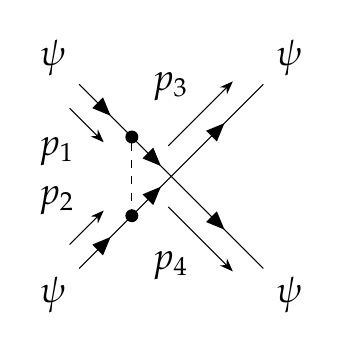
\begin{tikzpicture}[baseline=(current bounding box.center)]
  \begin{feynman}
    \vertex (i1) at (-1.5, 1.5) {$\psi$};
    \vertex (f1) at (1.5, 1.5) {$\psi$};
    \vertex (i2) at (-1.5, -1.5) {$\psi$};
    \vertex (f2) at (1.5, -1.5) {$\psi$};
    \vertex[dot] (v1) at (-0.5, 0.5) {};
    \vertex[dot] (v2) at (-0.5, -0.5) {};
    \vertex (v0) at (0,0);
    \draw[fermion, momentum'=$p_1$] (i1) -- (v1);
    \draw[fermion, momentum=$p_2$] (i2) -- (v2);
    \draw[fermion, momentum=$p_3$] (v0) -- (f1);
    \draw[fermion, momentum'=$p_4$] (v0) -- (f2);
    \draw[fermion] (v1) -- (v0);
    \draw[fermion] (v2) -- (v0);
    \draw[scalar] (v1) -- (v2);
  \end{feynman}
\end{tikzpicture}
\end{center}
1-loop diagrams (Self-Energies, Vertex Correction, Box):
\begin{center}
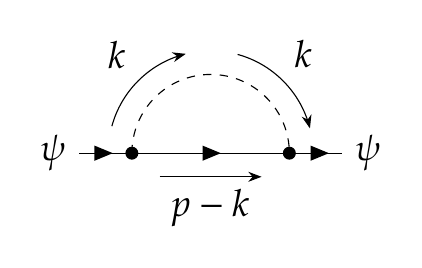
\begin{tikzpicture}[baseline=(current bounding box.center)]
  \begin{feynman}
    \vertex[dot] (v1) at (-1,0) {};
    \vertex[dot] (v2) at (1,0) {};
    \vertex (i1) at (-2,0) {$\psi$};
    \vertex (f1) at (2,0) {$\psi$};
    \draw[fermion] (i1) -- (v1);
    \draw[fermion, momentum'=$p-k$] (v1) -- (v2);
    \draw[fermion] (v2) -- (f1);
    \draw[scalar, momentum=$k$] (v1) arc[start angle=180, end angle=0, radius=1cm];
  \end{feynman}
\end{tikzpicture}
\hspace{1cm}
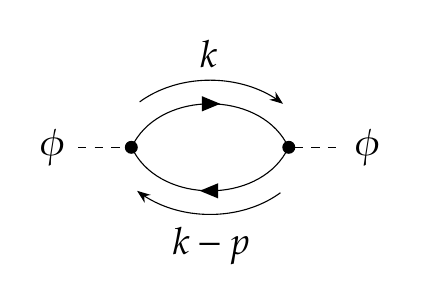
\begin{tikzpicture}[baseline=(current bounding box.center)]
  \begin{feynman}
    \vertex[dot] (v1) at (-1,0) {};
    \vertex[dot] (v2) at (1,0) {};
    \vertex (i1) at (-2,0) {$\phi$};
    \vertex (f1) at (2,0) {$\phi$};
    \draw[scalar] (i1) -- (v1);
    \draw[scalar] (v2) -- (f1);
    \draw[fermion, momentum=$k$] (v1) to[out=60, in=120] (v2);
    \draw[fermion, momentum=$k-p$] (v2) to[out=-120, in=-60] (v1);
  \end{feynman}
\end{tikzpicture}
\end{center}
\begin{center}
\begin{tikzpicture}[baseline=(current bounding box.center)]
  \begin{feynman}
    \vertex (v1) at (-0.5, 1);
    \vertex (v2) at (-0.5, -1);
    \vertex (v3) at (1, 0);
    \vertex (i1) at (-1, 2) {$\psi$};
    \vertex (i2) at (-1, -2) {$\psi$};
    \vertex (f2) at (2, 0) {$\phi$};
    \draw[scalar] (v1) -- (v2);
    \draw[fermion] (i2) -- (v2);
    \draw[fermion] (v2) -- (v3);
    \draw[fermion] (v3) -- (v1);
    \draw[fermion] (v1) -- (i1);
    \draw[scalar] (v3) -- (f2);
  \end{feynman}
\end{tikzpicture}
\hspace{1cm}
\begin{tikzpicture}[baseline=(current bounding box.center)]
  \begin{feynman}
    \vertex[dot] (v1) at (-1,-1) {};
    \vertex[dot] (v2) at (-1,1) {};
    \vertex[dot] (v3) at (1,1) {};
    \vertex[dot] (v4) at (1,-1) {};
    \vertex (i1) at (-2, -1.5) {$\psi$};
    \vertex (i2) at (-2, 1.5) {$\psi$};
    \vertex (f1) at (2, 1.5) {$\psi$};
    \vertex (f2) at (2, -1.5) {$\psi$};
    \draw[fermion] (i1) -- (v1);
    \draw[fermion] (i2) -- (v2);
    \draw[fermion] (v3) -- (f1);
    \draw[fermion] (v4) -- (f2);
    \draw[scalar] (v1) -- (v2);
    \draw[scalar] (v2) -- (v3);
    \draw[scalar] (v3) -- (v4);
    \draw[scalar] (v4) -- (v1);
  \end{feynman}
\end{tikzpicture}
\hspace{1cm}
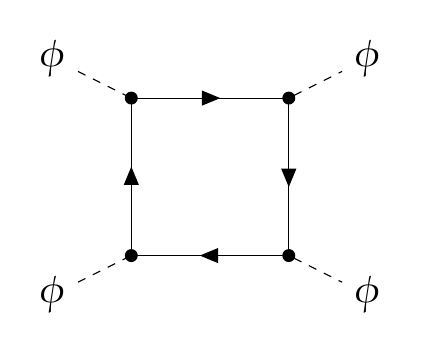
\begin{tikzpicture}[baseline=(current bounding box.center)]
  \begin{feynman}
    \vertex[dot] (v1) at (-1,-1) {};
    \vertex[dot] (v2) at (-1,1) {};
    \vertex[dot] (v3) at (1,1) {};
    \vertex[dot] (v4) at (1,-1) {};
    \vertex (i1) at (-2, -1.5) {$\phi$};
    \vertex (i2) at (-2, 1.5) {$\phi$};
    \vertex (f1) at (2, 1.5) {$\phi$};
    \vertex (f2) at (2, -1.5) {$\phi$};
    \draw[scalar] (i1) -- (v1);
    \draw[scalar] (i2) -- (v2);
    \draw[scalar] (v3) -- (f1);
    \draw[scalar] (v4) -- (f2);
    \draw[fermion] (v1) -- (v2);
    \draw[fermion] (v2) -- (v3);
    \draw[fermion] (v3) -- (v4);
    \draw[fermion] (v4) -- (v1);
  \end{feynman}
\end{tikzpicture}
\end{center}
Counter terms:
\begin{center}
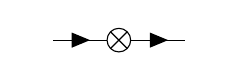
\begin{tikzpicture}[baseline=(current bounding box.center)]
  \begin{feynman}
    \vertex (v1) at (-1,0) {};
    \vertex (v2) at (1,0) {};
    \vertex[counterterm] (v0) at (0,0) {};
    \draw[fermion] (v1) -- (v0);
    \draw[fermion] (v0) -- (v2);
  \end{feynman}
\end{tikzpicture}
\hspace{1cm}
\begin{tikzpicture}[baseline=(current bounding box.center)]
  \begin{feynman}
    \vertex (v1) at (-1,0) {};
    \vertex (v2) at (1,0) {};
    \vertex[counterterm] (v0) at (0,0) {};
    \draw[scalar] (v1) -- (v0);
    \draw[scalar] (v0) -- (v2);
  \end{feynman}
\end{tikzpicture}
\hspace{1cm}
\begin{tikzpicture}[baseline=(current bounding box.center)]
  \begin{feynman}
    \vertex[counterterm] (v1) at (0,0) {};
    \vertex (i1) at (-0.7, 1.4) {$\psi$};
    \vertex (i2) at (-0.7, -1.4) {$\psi$};
    \vertex (f2) at (1.5, 0) {$\phi$};
    \draw[fermion] (v1) -- (i1);
    \draw[fermion] (i2) -- (v1);
    \draw[scalar] (v1) -- (f2);
  \end{feynman}
\end{tikzpicture}
\end{center}
\subsubsection*{Beta Function}
\begin{equation}
    \beta(g) = \frac{5g^3}{16\pi^2}
\end{equation}

\subsection{Fermion QED}
\subsubsection*{Full Bare Lagrangian}
(Includes Gauge Fixing term)
\begin{equation}
    \mathcal{L} = \bar{\psi}(i\slashed{D} - m)\psi - \frac{1}{4}F_{\mu\nu}F^{\mu\nu} - \frac{1}{2\xi}(\partial_\mu A^\mu)^2, \quad D_\mu = \partial_\mu + ieA_\mu
\end{equation}
\subsubsection*{Symmetries}
Poincar\'{e} invariance, Local $U(1)$ Gauge ($\psi \to e^{ie\alpha(x)}\psi$, $A_\mu \to A_\mu - \partial_\mu \alpha$), $C, P, T$ symmetries.
\subsubsection*{Equations of Motion}
\begin{equation}
    (i\slashed{D} - m)\psi = 0, \qquad \partial_\mu F^{\mu\nu} + \frac{1}{\xi}\partial^\nu(\partial_\mu A^\mu) = e\bar{\psi}\gamma^\nu\psi
\end{equation}
\subsubsection*{Superficial Degree of Divergence}
\begin{equation}
    D = 4 - \frac{3}{2}N_e - N_\gamma
\end{equation}
\subsubsection*{Gauge Fixing}
The naive photon propagator cannot be inverted because the kinetic operator $(q^2 \eta^{\mu\nu} - q^\mu q^\nu)$ has a zero eigenvalue reflecting gauge redundancy. Using the Faddeev-Popov procedure, we add a gauge-fixing term $-\frac{1}{2\xi}(\partial_\mu A^\mu)^2$, which enforces the Lorentz gauge condition $\partial_\mu A^\mu = 0$ in the path integral. The resulting general bare propagator is:
\begin{equation}
    D_F^{\mu\nu}(q) = \frac{-i}{q^2 + i\epsilon}\left(\eta^{\mu\nu} - (1 - \xi)\frac{q^\mu q^\nu}{q^2}\right)
\end{equation}
\textbf{Feynman Gauge} ($\xi = 1$): Eliminates the $q^\mu q^\nu$ term entirely, yielding $D_F^{\mu\nu}(q) = \frac{-i\eta^{\mu\nu}}{q^2 + i\epsilon}$. \\
\textbf{Landau Gauge} ($\xi = 0$): Enforces absolute transversality of the propagator, $D_F^{\mu\nu}(q) = \frac{-i}{q^2 + i\epsilon}\left(\eta^{\mu\nu} - \frac{q^\mu q^\nu}{q^2}\right)$.
\subsubsection*{Feynman rules}
\begin{itemize}
    \item Photon Propagator: $D_F^{\mu\nu}(p)$ (as defined above).
    \item Fermion Propagator: $\frac{i(\slashed{p}+m)}{p^2-m^2+i\epsilon}$
    \item QED Vertex: $-ie\gamma^\mu (2\pi)^4\delta^{(4)}(\sum p)$
\end{itemize}
\subsubsection*{Counter terms and Renormalized Lagrangian}
\begin{equation}
    \mathcal{L}_{CT} = i\delta_2 \bar{\psi}\slashed{\partial}\psi - \delta_m \bar{\psi}\psi - \frac{1}{4}\delta_3 (F_{\mu\nu})^2 - e\delta_1 \bar{\psi}\gamma^\mu A_\mu \psi
\end{equation}
\subsubsection*{On-Shell Renormalization}
We demand the physical electron mass $m$, physical field strength, and the macroscopic physical charge $e$:
\begin{equation}
    \Sigma_R(\slashed{p}=m_e) = 0, \qquad \left.\frac{d\Sigma_R}{d\slashed{p}}\right|_{\slashed{p}=m_e} = 0 \qquad \text{(Fixes } \delta_m, \delta_2 \text{)}
\end{equation}
\begin{equation}
    \Pi_R(q^2=0) = 0 \qquad \text{(Fixes } \delta_3 \text{, keeping photon massless)}
\end{equation}
\begin{equation}
    -ie\Gamma^\mu(q=0) = -ie\gamma^\mu \qquad \text{(Fixes } \delta_1 \text{ at threshold scattering limit)}
\end{equation}
\subsubsection*{Full Propagators}
After on-shell renormalization, the exact propagators are:
Fermion:
\begin{equation}
    S_{F,R}(p) = \frac{i}{\slashed{p} - m - \Sigma_R(\slashed{p})} \xrightarrow{p^2 \to m^2} \frac{i}{\slashed{p} - m + i\epsilon}
\end{equation}
Photon:
\begin{equation}
    D^{\mu\nu}_R(q) = \frac{-i}{q^2(1 - \Pi_R(q^2))} \left( \eta^{\mu\nu} - \frac{q^\mu q^\nu}{q^2} \right) - i\xi \frac{q^\mu q^\nu}{q^4} \xrightarrow{q^2 \to 0} \frac{-i\eta^{\mu\nu}}{q^2} + \text{gauge terms}
\end{equation}
\subsubsection*{Ward-Takahashi Identities}
The General WT Identity links the 3-point vertex correction to the fermion propagator:
\begin{equation}
    q_\mu \Gamma^\mu(p, p+q) = S_{F,R}^{-1}(p+q) - S_{F,R}^{-1}(p)
\end{equation}
Taking the limit $q \to 0$ enforces $Z_1 = Z_2$ (and thus $\delta_1 = \delta_2$). This ensures the physical charge $e$ is renormalized identically for all species uniquely by the vacuum polarization $Z_3$. Furthermore, gauge invariance mandates the transversality of the Photon Self-Energy: $q_\mu \Pi^{\mu\nu}(q) = 0$.
\subsubsection*{Interactions \& Correlation Functions}
\begin{itemize}
    \item \textbf{3-point (Furry's Theorem):} The 3-photon vertex $\langle \Omega | T A_\mu(x) A_\nu(y) A_\rho(z) | \Omega \rangle = 0$ is identically zero due to Charge Conjugation symmetry. Any closed fermion loop with an odd number of photon vertices vanishes.
    \item \textbf{3-point (Vertex):} The fermion-photon vertex $\langle \psi \bar{\psi} A_\mu \rangle$ yields the dressed vertex $\Gamma^\mu(p',p) = \gamma^\mu F_1(q^2) + \frac{i\sigma^{\mu\nu}q_\nu}{2m} F_2(q^2)$. Anomalous magnetic moment $a_e = \frac{g-2}{2} = F_2(0) = \frac{\alpha}{2\pi}$.
    \item \textbf{Vacuum Polarization:} $\Pi^{\mu\nu}(q) = (q^2\eta^{\mu\nu} - q^\mu q^\nu)\Pi(q^2)$.
    \item \textbf{Møller Scattering ($e^- e^- \to e^- e^-$):} $t$ and $u$ channel photon exchange.
    \item \textbf{Bhabha Scattering ($e^- e^+ \to e^- e^+$):} $s$ and $t$ channel photon exchange.
    \item \textbf{Compton Scattering ($e^- \gamma \to e^- \gamma$):} $s$ and $u$ channel fermion exchange.
\end{itemize}
\subsubsection*{Diagrams}
Tree $2 \to 2$ scattering (Møller $e^- e^- \to e^- e^-$), T and U channels:
\begin{center}
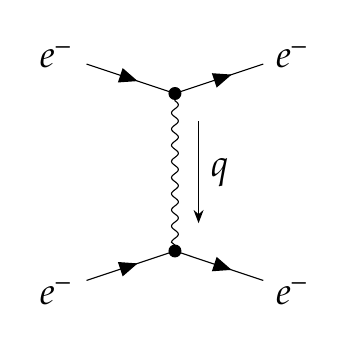
\begin{tikzpicture}[baseline=(current bounding box.center)]
  \begin{feynman}
    \vertex[dot] (v1) at (0,1) {};
    \vertex[dot] (v2) at (0,-1) {};
    \vertex (i1) at (-1.5, 1.5) {$e^-$};
    \vertex (f1) at (1.5, 1.5) {$e^-$};
    \vertex (i2) at (-1.5, -1.5) {$e^-$};
    \vertex (f2) at (1.5, -1.5) {$e^-$};
    \draw[fermion] (i1) -- (v1);
    \draw[fermion] (v1) -- (f1);
    \draw[fermion] (i2) -- (v2);
    \draw[fermion] (v2) -- (f2);
    \draw[photon, momentum=$q$] (v1) -- (v2);
  \end{feynman}
\end{tikzpicture}
\hspace{1cm}
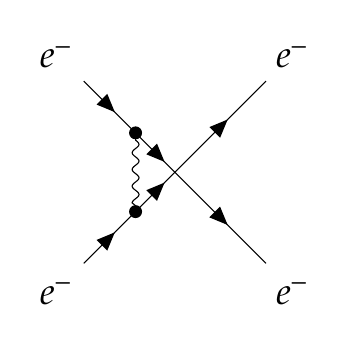
\begin{tikzpicture}[baseline=(current bounding box.center)]
  \begin{feynman}
    \vertex (i1) at (-1.5, 1.5) {$e^-$};
    \vertex (f1) at (1.5, 1.5) {$e^-$};
    \vertex (i2) at (-1.5, -1.5) {$e^-$};
    \vertex (f2) at (1.5, -1.5) {$e^-$};
    \vertex[dot] (v1) at (-0.5, 0.5) {};
    \vertex[dot] (v2) at (-0.5, -0.5) {};
    \vertex (v0) at (0,0);
    \draw[fermion] (i1) -- (v1);
    \draw[fermion] (i2) -- (v2);
    \draw[fermion] (v0) -- (f1);
    \draw[fermion] (v0) -- (f2);
    \draw[fermion] (v1) -- (v0);
    \draw[fermion] (v2) -- (v0);
    \draw[photon] (v1) -- (v2);
  \end{feynman}
\end{tikzpicture}
\end{center}
Tree $2 \to 2$ scattering (Bhabha $e^- e^+ \to e^- e^+$), S and T channels:
\begin{center}
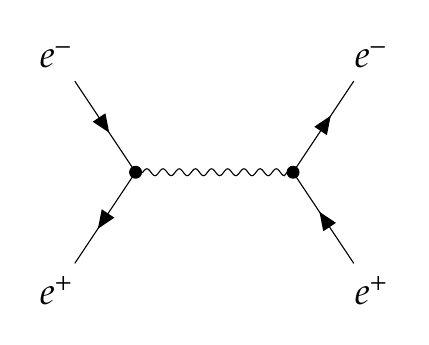
\begin{tikzpicture}[baseline=(current bounding box.center)]
  \begin{feynman}
    \vertex[dot] (v1) at (-1,0) {};
    \vertex[dot] (v2) at (1,0) {};
    \vertex (i1) at (-2, 1.5) {$e^-$};
    \vertex (i2) at (-2, -1.5) {$e^+$};
    \vertex (f1) at (2, 1.5) {$e^-$};
    \vertex (f2) at (2, -1.5) {$e^+$};
    \draw[fermion] (i1) -- (v1);
    \draw[fermion] (v1) -- (i2);
    \draw[photon] (v1) -- (v2);
    \draw[fermion] (v2) -- (f1);
    \draw[fermion] (f2) -- (v2);
  \end{feynman}
\end{tikzpicture}
\hspace{1cm}
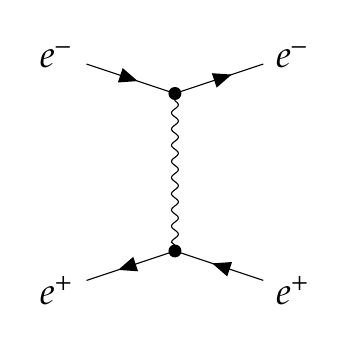
\begin{tikzpicture}[baseline=(current bounding box.center)]
  \begin{feynman}
    \vertex[dot] (v1) at (0,1) {};
    \vertex[dot] (v2) at (0,-1) {};
    \vertex (i1) at (-1.5, 1.5) {$e^-$};
    \vertex (f1) at (1.5, 1.5) {$e^-$};
    \vertex (i2) at (-1.5, -1.5) {$e^+$};
    \vertex (f2) at (1.5, -1.5) {$e^+$};
    \draw[fermion] (i1) -- (v1);
    \draw[fermion] (v1) -- (f1);
    \draw[fermion] (f2) -- (v2);
    \draw[fermion] (v2) -- (i2);
    \draw[photon] (v1) -- (v2);
  \end{feynman}
\end{tikzpicture}
\end{center}
Tree $2 \to 2$ scattering (Compton $e^- \gamma \to e^- \gamma$), S and U channels:
\begin{center}
\begin{tikzpicture}[baseline=(current bounding box.center)]
  \begin{feynman}
    \vertex[dot] (v1) at (-1,0) {};
    \vertex[dot] (v2) at (1,0) {};
    \vertex (i1) at (-2, -1.5) {$e^-$};
    \vertex (i2) at (-2, 1.5) {$\gamma$};
    \vertex (f1) at (2, 1.5) {$e^-$};
    \vertex (f2) at (2, -1.5) {$\gamma$};
    \draw[fermion] (i1) -- (v1);
    \draw[photon] (i2) -- (v1);
    \draw[fermion] (v1) -- (v2);
    \draw[fermion] (v2) -- (f1);
    \draw[photon] (v2) -- (f2);
  \end{feynman}
\end{tikzpicture}
\hspace{1cm}
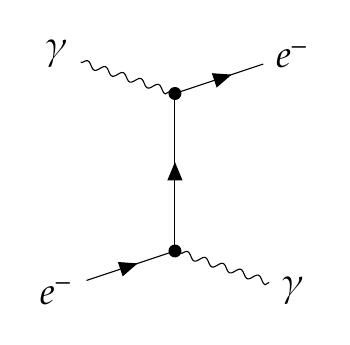
\begin{tikzpicture}[baseline=(current bounding box.center)]
  \begin{feynman}
    \vertex[dot] (v1) at (0,-1) {};
    \vertex[dot] (v2) at (0,1) {};
    \vertex (i1) at (-1.5, -1.5) {$e^-$};
    \vertex (i2) at (-1.5, 1.5) {$\gamma$};
    \vertex (f1) at (1.5, -1.5) {$\gamma$};
    \vertex (f2) at (1.5, 1.5) {$e^-$};
    \draw[fermion] (i1) -- (v1);
    \draw[photon] (i2) -- (v2);
    \draw[photon] (v1) -- (f1);
    \draw[fermion] (v2) -- (f2);
    \draw[fermion] (v1) -- (v2);
  \end{feynman}
\end{tikzpicture}
\end{center}
1-loop diagrams (Electron Self-Energy, Vacuum Polarization, Vertex Correction):
\begin{center}
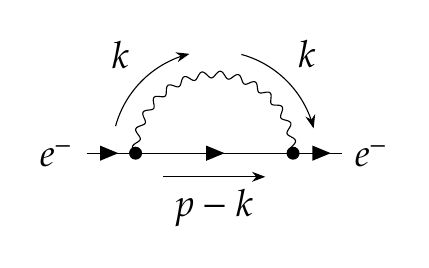
\begin{tikzpicture}[baseline=(current bounding box.center)]
  \begin{feynman}
    \vertex[dot] (v1) at (-1,0) {};
    \vertex[dot] (v2) at (1,0) {};
    \vertex (i1) at (-2,0) {$e^-$};
    \vertex (f1) at (2,0) {$e^-$};
    \draw[fermion] (i1) -- (v1);
    \draw[fermion, momentum'=$p-k$] (v1) -- (v2);
    \draw[fermion] (v2) -- (f1);
    \draw[photon, momentum=$k$] (v1) arc[start angle=180, end angle=0, radius=1cm];
  \end{feynman}
\end{tikzpicture}
\hspace{0.5cm}
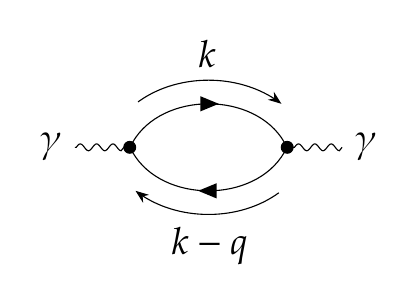
\begin{tikzpicture}[baseline=(current bounding box.center)]
  \begin{feynman}
    \vertex[dot] (v1) at (-1,0) {};
    \vertex[dot] (v2) at (1,0) {};
    \vertex (i1) at (-2,0) {$\gamma$};
    \vertex (f1) at (2,0) {$\gamma$};
    \draw[photon] (i1) -- (v1);
    \draw[photon] (v2) -- (f1);
    \draw[fermion, momentum=$k$] (v1) to[out=60, in=120] (v2);
    \draw[fermion, momentum=$k-q$] (v2) to[out=-120, in=-60] (v1);
  \end{feynman}
\end{tikzpicture}
\hspace{0.5cm}
\begin{tikzpicture}[baseline=(current bounding box.center)]
  \begin{feynman}
    \vertex (v1) at (-0.5, 1);
    \vertex (v2) at (-0.5, -1);
    \vertex (v3) at (1, 0);
    \vertex (i1) at (-1, 2) {$e^-$};
    \vertex (i2) at (-1, -2) {$e^-$};
    \vertex (f2) at (2, 0) {$\gamma$};
    \draw[photon] (v1) -- (v2);
    \draw[fermion] (i2) -- (v2);
    \draw[fermion] (v2) -- (v3);
    \draw[fermion] (v3) -- (v1);
    \draw[fermion] (v1) -- (i1);
    \draw[photon] (v3) -- (f2);
  \end{feynman}
\end{tikzpicture}
\end{center}
\subsubsection*{Beta Function}
\begin{equation}
    \beta(e) = \frac{e^3}{12\pi^2}
\end{equation}
\subsubsection*{IR Divergences and Bremsstrahlung}
When an electrically charged particle undergoes scattering, the probability of emitting a very low-energy (soft) photon (Bremsstrahlung) diverges. The cross-section for emitting a photon with energy less than some detector resolution $E_{\text{cut}}$ diverges logarithmically at the lower bound (as $\mu_{IR} \to 0$): 
\begin{equation}
    \sigma_{\text{Brem}} \propto \alpha \int_{\mu_{IR}}^{E_{\text{cut}}} \frac{dE_\gamma}{E_\gamma} \sim \alpha \ln\left(\frac{E_{\text{cut}}}{\mu_{IR}}\right)
\end{equation}
Simultaneously, the 1-loop virtual vertex correction $F_1(q^2)$ generates a negative logarithmic divergence of the exact same form due to soft virtual photons in the loop. 
\newline
\textbf{The Bloch-Nordsieck Theorem:} Any physical detector has a finite energy resolution $E_{\text{cut}}$, meaning it cannot distinguish between a pure elastic scattering event and an inelastic scattering event where an unobservably soft photon is emitted. The physically measurable cross section is the sum:
\begin{equation}
    \sigma_{\text{obs}} = \sigma_{\text{virtual}} + \sigma_{\text{Brem}}
\end{equation}
In this sum, the IR divergence $\ln(\mu_{IR})$ perfectly cancels out to all orders in perturbation theory, leaving a finite, observable result that depends only on the detector's cutoff $E_{\text{cut}}$.

\subsection{Scalar QED}
\subsubsection*{Full Bare Lagrangian}
(Includes quartic $(\phi^\dagger \phi)^2$ term required for renormalization, and gauge fixing).
\begin{equation}
    \mathcal{L} = (D_\mu \phi)^\dagger (D^\mu \phi) - m^2\phi^\dagger \phi - \frac{\lambda}{4}(\phi^\dagger \phi)^2 - \frac{1}{4}F_{\mu\nu}F^{\mu\nu} - \frac{1}{2\xi}(\partial_\mu A^\mu)^2
\end{equation}
\subsubsection*{Symmetries}
Poincar\'{e} invariance, Local $U(1)$ Gauge ($\phi \to e^{ie\alpha(x)}\phi$, $A_\mu \to A_\mu - \partial_\mu \alpha$), $C, P, T$ symmetries.
\subsubsection*{Equations of Motion}
\begin{equation}
    D_\mu D^\mu \phi + m^2\phi + \frac{\lambda}{2}(\phi^\dagger \phi)\phi = 0, \qquad \partial_\mu F^{\mu\nu} + \frac{1}{\xi}\partial^\nu(\partial_\mu A^\mu) = ie(\phi^\dagger D^\nu \phi - (D^\nu\phi^\dagger)\phi)
\end{equation}
\subsubsection*{Superficial Degree of Divergence}
\begin{equation}
    D = 4 - N_\phi - N_\gamma
\end{equation}
\subsubsection*{Feynman rules}
\begin{itemize}
    \item Cubic Vertex ($A_\mu \phi^\dagger \phi$): $-ie(p + p')^\mu$ (where $p, p'$ are incoming/outgoing scalar momenta)
    \item Quartic (Seagull) Vertex ($A_\mu A_\nu \phi^\dagger \phi$): $2ie^2\eta^{\mu\nu}$
\end{itemize}
\subsubsection*{Counter terms and Renormalized Lagrangian}
\begin{equation}
    \mathcal{L}_{CT} = \delta_Z |D_\mu \phi|^2 - \delta_m |\phi|^2 - \frac{\delta_\lambda}{4}|\phi|^4 - \frac{1}{4}\delta_A (F_{\mu\nu})^2
\end{equation}
By gauge invariance, the counterterms for the cubic vertex ($-ie\delta_1(p+p')^\mu$) and quartic vertex ($2ie^2\delta_2\eta^{\mu\nu}$) are strictly fixed to match the field renormalization: $\delta_1 = \delta_2 = \delta_Z$.
\subsubsection*{On-Shell Renormalization}
We apply identical on-shell conditions as in Fermion QED to fix the scalar mass $m$, maintain a massless photon, and fix the charge $e$:
\begin{equation}
    \Sigma_R(m^2) = 0, \qquad \left.\frac{d\Sigma_R}{dp^2}\right|_{p^2=m^2} = 0, \qquad \Pi_R(0) = 0
\end{equation}
\subsubsection*{Full Propagators}
After on-shell renormalization, the exact propagators are:
Scalar:
\begin{equation}
    D_{F,R}(p) = \frac{i}{p^2 - m^2 - \Sigma_R(p^2)} \xrightarrow{p^2 \to m^2} \frac{i}{p^2 - m^2 + i\epsilon}
\end{equation}
Photon: (Identical to Fermion QED).
\subsubsection*{Ward-Takahashi Identities}
Analogous to Fermion QED, ensuring charge conservation and transversality of the photon self-energy tensor $\Pi^{\mu\nu}(q)$.
\begin{equation}
    q_\mu \Gamma^\mu(p, p+q) = \Delta_{F,R}^{-1}(p+q) - \Delta_{F,R}^{-1}(p)
\end{equation}
\subsubsection*{Interactions \& Correlation Functions}
\begin{itemize}
    \item \textbf{1-point:} Gauge invariance prohibits scalar tadpoles $\langle \phi \rangle = 0$.
    \item \textbf{3-point (Furry's Theorem analog):} The 3-photon vertex $\langle A_\mu A_\nu A_\rho \rangle = 0$ by Charge Conjugation symmetry. 
    \item \textbf{3-point (Vertex):} The fundamental 3-point function is the scalar-photon vertex $\langle \phi^\dagger \phi A_\mu \rangle$, yielding the dressed vertex $\Gamma^\mu(p',p)$.
    \item \textbf{$2 \to 2$ Scattering:} Compton scattering $\gamma \phi \to \gamma \phi$ proceeds via $s$ and $u$ channels (cubic vertex) PLUS a contact term from the quartic seagull vertex. This seagull diagram is strictly necessary to satisfy gauge invariance and the Ward Identity.
\end{itemize}
\subsubsection*{Diagrams}
Vertices:
\begin{center}
\begin{tikzpicture}[baseline=(current bounding box.center)]
  \begin{feynman}
    \vertex[dot] (v1) at (-1,0) {};
    \vertex (i1) at (-2, -1.5) {$\phi$};
    \vertex (i2) at (-2, 1.5) {$\phi$};
    \vertex (f1) at (1.5, 0) {$\gamma$};
    \draw[charged scalar] (i1) -- (v1);
    \draw[charged scalar] (v1) -- (i2);
    \draw[photon] (v1) -- (f1);
  \end{feynman}
\end{tikzpicture}
\hspace{0.5cm}
\begin{tikzpicture}[baseline=(current bounding box.center)]
  \begin{feynman}
    \vertex[dot] (v1) at (0,0) {};
    \vertex (i1) at (-1.5, -1.5) {$\phi$};
    \vertex (i2) at (-1.5, 1.5) {$\gamma$};
    \vertex (f1) at (1.5, -1.5) {$\gamma$};
    \vertex (f2) at (1.5, 1.5) {$\phi$};
    \draw[photon] (i1) -- (v1);
    \draw[photon] (v1) -- (i2);
    \draw[charged scalar] (f1) -- (v1);
    \draw[charged scalar] (v1) -- (f2);
  \end{feynman}
\end{tikzpicture}
\end{center}
Tree $2 \to 2$ scattering (Compton $\gamma \phi \to \gamma \phi$), S, U, and Seagull channels:
\begin{center}
\begin{tikzpicture}[baseline=(current bounding box.center)]
  \begin{feynman}
    \vertex[dot] (v1) at (-1,0) {};
    \vertex[dot] (v2) at (1,0) {};
    \vertex (i1) at (-2, -1.5) {$\phi$};
    \vertex (i2) at (-2, 1.5) {$\gamma$};
    \vertex (f1) at (2, 1.5) {$\phi$};
    \vertex (f2) at (2, -1.5) {$\gamma$};
    \draw[charged scalar] (i1) -- (v1);
    \draw[photon] (i2) -- (v1);
    \draw[charged scalar] (v1) -- (v2);
    \draw[charged scalar] (v2) -- (f1);
    \draw[photon] (v2) -- (f2);
  \end{feynman}
\end{tikzpicture}
\hspace{0.5cm}
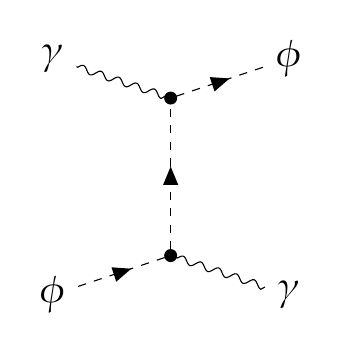
\begin{tikzpicture}[baseline=(current bounding box.center)]
  \begin{feynman}
    \vertex[dot] (v1) at (0,-1) {};
    \vertex[dot] (v2) at (0,1) {};
    \vertex (i1) at (-1.5, -1.5) {$\phi$};
    \vertex (i2) at (-1.5, 1.5) {$\gamma$};
    \vertex (f1) at (1.5, -1.5) {$\gamma$};
    \vertex (f2) at (1.5, 1.5) {$\phi$};
    \draw[charged scalar] (i1) -- (v1);
    \draw[photon] (i2) -- (v2);
    \draw[photon] (v1) -- (f1);
    \draw[charged scalar] (v2) -- (f2);
    \draw[charged scalar] (v1) -- (v2);
  \end{feynman}
\end{tikzpicture}
\hspace{0.5cm}
\begin{tikzpicture}[baseline=(current bounding box.center)]
  \begin{feynman}
    \vertex[dot] (v) at (0,0) {};
    \vertex (i1) at (-1.5, -1.5) {$\phi$};
    \vertex (i2) at (-1.5, 1.5) {$\gamma$};
    \vertex (f1) at (1.5, 1.5) {$\gamma$};
    \vertex (f2) at (1.5, -1.5) {$\phi$};
    \draw[charged scalar] (i1) -- (v);
    \draw[photon] (i2) -- (v);
    \draw[charged scalar] (v) -- (f1);
    \draw[photon] (v) -- (f2);
  \end{feynman}
\end{tikzpicture}
\end{center}
1-loop diagrams (Vacuum Polarization, Scalar Self-Energy Photon Loop, Seagull Tadpole):
\begin{center}
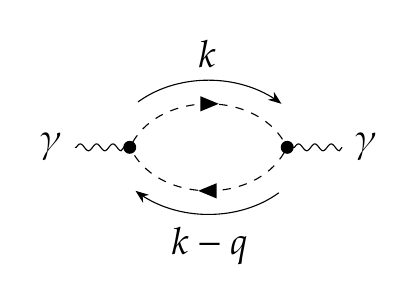
\begin{tikzpicture}[baseline=(current bounding box.center)]
  \begin{feynman}
    \vertex[dot] (v1) at (-1,0) {};
    \vertex[dot] (v2) at (1,0) {};
    \vertex (i1) at (-2,0) {$\gamma$};
    \vertex (f1) at (2,0) {$\gamma$};
    \draw[photon] (i1) -- (v1);
    \draw[photon] (v2) -- (f1);
    \draw[charged scalar, momentum=$k$] (v1) to[out=60, in=120] (v2);
    \draw[charged scalar, momentum=$k-q$] (v2) to[out=-120, in=-60] (v1);
  \end{feynman}
\end{tikzpicture}
\hspace{0.5cm}
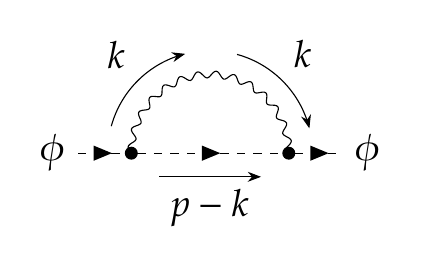
\begin{tikzpicture}[baseline=(current bounding box.center)]
  \begin{feynman}
    \vertex[dot] (v1) at (-1,0) {};
    \vertex[dot] (v2) at (1,0) {};
    \vertex (i1) at (-2,0) {$\phi$};
    \vertex (f1) at (2,0) {$\phi$};
    \draw[charged scalar] (i1) -- (v1);
    \draw[charged scalar, momentum'=$p-k$] (v1) -- (v2);
    \draw[charged scalar] (v2) -- (f1);
    \draw[photon, momentum=$k$] (v1) arc[start angle=180, end angle=0, radius=1cm];
  \end{feynman}
\end{tikzpicture}
\hspace{0.5cm}
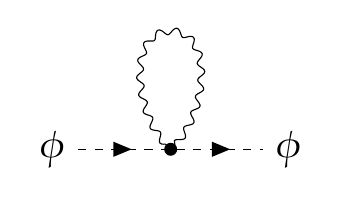
\begin{tikzpicture}[baseline=(current bounding box.center)]
  \begin{feynman}
    \vertex[dot] (a) at (0,0) {};
    \vertex (i1) at (-1.5, 0) {$\phi$};
    \vertex (f1) at (1.5, 0) {$\phi$};
    \vertex (loop_top) at (0, 1.5);
    \draw[charged scalar] (i1) -- (a);
    \draw[charged scalar] (a) -- (f1);
    \draw[photon] (a) to[out=135, in=180] (loop_top) to[out=0, in=45] (a);
  \end{feynman}
\end{tikzpicture}
\hspace{0.5cm}
\begin{tikzpicture}[baseline=(current bounding box.center)]
  \begin{feynman}
    \vertex (v1) at (-0.5, 1);
    \vertex (v2) at (-0.5, -1);
    \vertex (v3) at (1, 0);
    \vertex (i1) at (-1, 2) {$e^-$};
    \vertex (i2) at (-1, -2) {$e^-$};
    \vertex (f2) at (2, 0) {$\gamma$};
    \draw[photon] (v1) -- (v2);
    \draw[charged scalar] (i2) -- (v2);
    \draw[charged scalar] (v2) -- (v3);
    \draw[charged scalar] (v3) -- (v1);
    \draw[charged scalar] (v1) -- (i1);
    \draw[photon] (v3) -- (f2);
  \end{feynman}
\end{tikzpicture}
\end{center}
\subsubsection*{Beta Function}
\begin{equation}
    \beta(e) = \frac{e^3}{48\pi^2}
\end{equation}
(The scalar loop contribution to vacuum polarization is 1/4 that of a Dirac fermion).
\newpage
\section{Math}
\subsection{Gaussian Integrals}
Simple Gaussian:
\begin{equation}
    \int dx  e^{-ax^2 + bx} = \sqrt{\frac{\pi}{a}}e^{\frac{b^2}{2a}}
\end{equation}
$N$-dimensional, with source $J$:
\begin{equation}
    \int d^n x  e^{-\frac{1}{2} x^T A x + J^T x} = \sqrt{\frac{(2\pi)^N}{\det A}} \exp\left( \frac{1}{2} J^T A^{-1} J \right)
\end{equation}
Grassmann Numbers (assuming standard anticommutation $\theta_i \theta_j = -\theta_j \theta_i$):
\begin{equation}
    \int \left( \prod_{i=1}^N d\bar{\theta}_i d\theta_i \right) \exp\left( -\bar{\theta} M \theta + \bar{\eta}\theta + \bar{\theta}\eta \right) = (\det M) \exp\left( \bar{\eta} M^{-1} \eta \right)
\end{equation}
Functional Gaussian (fields path integral in continuous spacetime):
\begin{equation}
\begin{gathered}
    \int \mathcal{D}\phi \, \exp\left( -\frac{1}{2} \int d^4x \, d^4y \, \phi(x)A(x,y)\phi(y) + \int d^4x \, J(x)\phi(x) \right) \propto \\ \propto (\det A)^{-1/2} \exp\left( \frac{1}{2} \int d^4x \, d^4y \, J(x)A^{-1}(x,y)J(y) \right)
\end{gathered}
\end{equation}
\subsection{Feynman's trick}
Two variables:
\begin{equation}
    \frac{1}{AB} = \int_0^1 dx \int_0^1 dy \frac{\delta(x+y-1)}{[xA+yB]^2} = \int_0^1 dx \frac{1}{[xA + (1-x)B]^2}
\end{equation}
Three variables:
\begin{equation}
\begin{gathered}
    \frac{1}{ABC} = 2 \int_0^1 dx \int_0^1 dy \int_0^1 dz \frac{\delta(x+y+z-1)}{[xA+yB+zC]^3} = \\ = 2 \int_0^1 dx \int_0^{1-x} dy \frac{1}{[xA+yB+(1-x-y)C]^3}
\end{gathered}
\end{equation}
General:
\begin{equation}
    \frac{1}{A_1 \dots A_n} = (n-1)! \int_0^1 dx_1 \dots dx_n \delta\left(1 - \sum x_i\right) \frac{1}{(x_1 A_1 + \dots + x_n A_n)^n}
\end{equation}
\subsection{Grassman Numbers}
Definition:
A set of elements $\theta_i$ that completely anticommute: $\{\theta_i, \theta_j\} = \theta_i \theta_j + \theta_j \theta_i = 0$.
General term in the Grassman algebra of $n$ Grassman numbers $\theta_i$:
Because $\theta_i^2 = 0$, any function has a finite Taylor series. For 2 variables: $f(\theta_1, \theta_2) = A + B\theta_1 + C\theta_2 + D\theta_1\theta_2$.
\newline
Properties:
\begin{itemize}
    \item Nilpotency: $\theta_i^2 = 0$.
    \item Commute with normal c-numbers, anticommute with other Grassmanns.
\end{itemize}
Some basic functions:
\begin{align}
    e^\theta &= 1 + \theta \\
    \cos\theta &= 1, \quad \sin\theta = \theta \\
    \cosh\theta &= 1, \quad \sinh\theta = \theta
\end{align}
Differentiation and Integration:
Left differentiation: $\frac{\partial}{\partial \theta_i} (\theta_i \theta_j) = \theta_j$.
Integration rules (Berezin integral):
\begin{equation}
    \int d\theta = 0, \quad \int \theta d\theta = 1
\end{equation}
Delta function:
$\delta(\theta) = \theta$.
Complex Grassman numbers:
Formed by linear combinations: $\theta = \frac{1}{\sqrt{2}}(\theta_1 + i\theta_2)$, $\bar{\theta} = \frac{1}{\sqrt{2}}(\theta_1 - i\theta_2)$. Real Grassmann variables describe neutral fermions (Majorana), while complex describe charged fermions (Dirac). Conjugation reverses order: $(\theta \eta)^* = \eta^* \theta^*$.
Gaussian Integrals:
\begin{equation}
    \int d\bar{\theta} d\theta \, e^{-a\bar{\theta}\theta} = \int d\bar{\theta} d\theta \, (1 - a\bar{\theta}\theta) = a
\end{equation}
\subsection{Pauli matrices}
Definition:
\begin{equation}
    \sigma_1 = \begin{pmatrix} 0 & 1 \\ 1 & 0 \end{pmatrix}, \quad \sigma_2 = \begin{pmatrix} 0 & -i \\ i & 0 \end{pmatrix}, \quad \sigma_3 = \begin{pmatrix} 1 & 0 \\ 0 & -1 \end{pmatrix}
\end{equation}
Properties:
\begin{equation}
    [\sigma_i, \sigma_j] = 2i\epsilon_{ijk}\sigma_k, \quad \{\sigma_i, \sigma_j\} = 2\delta_{ij}\mathbb{1}, \quad \text{Tr}(\sigma_i) = 0
\end{equation}
\subsection{Gamma matrices}
Matrices satisfying the Dirac/Clifford algebra: $\{\gamma^\mu, \gamma^\nu\} = 2\eta^{\mu\nu}\mathbb{1}_{4\times 4}$.
Properties:
\begin{align}
    \text{Tr}(\mathbb{1}) &= 4 \\
    \text{Tr}(\text{any odd number of } \gamma) &= 0 \\
    \text{Tr}(\gamma^\mu \gamma^\nu) &= 4\eta^{\mu\nu} \\
    \text{Tr}(\gamma^\mu \gamma^\nu \gamma^\rho \gamma^\sigma) &= 4(\eta^{\mu\nu}\eta^{\rho\sigma} - \eta^{\mu\rho}\eta^{\nu\sigma} + \eta^{\mu\sigma}\eta^{\nu\rho}) \\
    \gamma^\mu \gamma_\mu &= 4 \\
    \gamma^\mu \slashed{a} \gamma_\mu &= -2\slashed{a}
\end{align}
\subsection{Inverting Fourier series}
If $f(x) = \sum_{k} e^{ikx} c_k$, then $c_k = \frac{1}{L} \int_0^L f(x) e^{-ikx} dx$.
\subsection{Fourier transform}
\begin{equation}
    f(x) = \int \frac{d^4k}{(2\pi)^4} e^{-ik\cdot x} \tilde{f}(k), \quad \tilde{f}(k) = \int d^4x e^{ik\cdot x} f(x)
\end{equation}
\subsection{Principal value}
Used in contour integration for resolving poles on the real axis:
\begin{equation}
    \lim_{\epsilon \to 0} \frac{1}{x \pm i\epsilon} = \mathcal{P}\left(\frac{1}{x}\right) \mp i\pi \delta(x)
\end{equation}
\subsection{Gamma function}
Definition:
\begin{equation}
    \Gamma(z) = \int_0^\infty x^{z-1} e^{-x} dx \quad (\text{for } \text{Re}(z) > 0)
\end{equation}
Properties:
\begin{align}
    \Gamma(z+1) &= z\Gamma(z) \\
    \Gamma(n) &= (n-1)! \quad (\text{for integer } n) \\
    \Gamma(1/2) &= \sqrt{\pi}
\end{align}
It has simple poles at $z = 0, -1, -2, \dots$ with residue $\frac{(-1)^n}{n!}$.
\subsection{The Residue Theorem}
If $f(z)$ is analytic inside and on some closed contour $C$ except at a finite number of isolated singularities $a_k$ inside $C$:
\begin{equation}
    \oint_C f(z) dz = 2\pi i \sum_{k=1}^n \text{Res}(f, a_k)
\end{equation}
where for a simple pole, the residue is $\text{Res}(f, c) = \lim_{z \to c} (z-c)f(z)$.
\end{document}